\documentclass[12pt,a4paper]{article}

\usepackage{xeCJK}
\setCJKmainfont{SimSun}[BoldFont=SimHei, ItalicFont=KaiTi]
\setCJKsansfont{SimHei}
\setCJKmonofont{FangSong}

% 中文编号支持
\usepackage{zhnumber}

\providecommand{\CJKrmdefault}{rm}
\providecommand{\CJKsfdefault}{sf}
\providecommand{\CJKttdefault}{tt}
\providecommand{\CJKfamilydefault}{\CJKrmdefault}

\usepackage{geometry}
\geometry{top=2.5cm,bottom=2.5cm,left=2.5cm,right=2.5cm}
\usepackage{amsmath,amssymb,amsfonts}
\usepackage{graphicx}
\graphicspath{{figures/}}
\usepackage{booktabs}
\usepackage{float}
\usepackage{caption}
\usepackage{subcaption}
\usepackage{listings}
\usepackage{color}
\usepackage{fancyhdr}
\usepackage{array}
\usepackage{longtable}
\usepackage{titlesec}
\usepackage{url}
\usepackage{hyperref}
\usepackage{enumitem}

\setlength{\headheight}{14.5pt}
\renewcommand{\baselinestretch}{1.38}
\renewcommand{\figurename}{图}
\renewcommand{\tablename}{表}

\titleformat{\section}{\zihao{4}\bfseries\heiti}{\thesection}{1em}{}
\titleformat{\subsection}{\zihao{-4}\bfseries\heiti}{\thesubsection}{1em}{}
\titleformat{\subsubsection}{\zihao{-4}\bfseries\heiti}{\thesubsubsection}{1em}{}
\captionsetup{font=small,labelfont=bf}

\definecolor{dkgreen}{rgb}{0,0.6,0}
\definecolor{gray}{rgb}{0.5,0.5,0.5}
\definecolor{mauve}{rgb}{0.58,0,0.82}
\lstset{frame=tb, language=Python, aboveskip=3mm, belowskip=3mm,
  showstringspaces=false, columns=flexible, basicstyle={\small\ttfamily},
  numbers=none, keywordstyle=\color{blue}, commentstyle=\color{dkgreen},
  stringstyle=\color{mauve}, breaklines=true, tabsize=3}

\title{\zihao{2}\bfseries 烟幕干扰弹的投放策略研究}
\author{}
\date{}

\titleformat{\section}{\zihao{4}\bfseries\heiti}{}{0em}{}
\titleformat{\subsection}{\zihao{-4}\bfseries\heiti}{}{0em}{}
\titleformat{\subsubsection}{\zihao{-4}\bfseries\heiti}{}{0em}{}
\begin{document}
\maketitle

% ==================== 摘要 ====================
\begin{center}
{\zihao{4}\bfseries 摘\quad 要}
\end{center}

\noindent 烟幕干扰弹通过在来袭导弹与保护目标之间形成烟幕遮蔽，干扰导弹对真目标的探测与打击。本文针对无人机投放烟幕干扰弹的策略优化问题，建立了运动学建模、几何遮蔽判定与混合整数非线性优化三层模型体系，通过粒子群优化与分层策略求解了五种递进场景下的最优投放方案。

\noindent \textbf{针对问题一}，建立了导弹、无人机、烟幕弹及云团的分段运动学方程，并提出基于"遮蔽视锥"的严格几何判定模型：以导弹为顶点、烟幕云团球为内切球构成圆锥，通过证明"圆柱被完全遮蔽当且仅当上下底面圆周全部落在视锥内"将三维判定降维为二维。采用离散时间步进法（$\Delta t=0.001$\,s）数值积分，求得有效遮蔽时长为 \textbf{1.392s}，验证了模型正确性。

\noindent \textbf{针对问题二}，以无人机航向角$\theta$、飞行速度$v$、投放时刻$t_{rel}$、引信延迟$\Delta t$为决策变量，建立遮蔽时长最大化的优化模型。采用粒子群算法（PSO）全局搜索与局部精修相结合的混合策略，求得最大有效遮蔽时长为 \textbf{4.578s}。

\noindent \textbf{针对问题三}，扩展为3枚烟幕弹的时序接力优化问题，决策变量增至8维。采用分层优化策略，以问题二最优解为初始方案，联合PSO搜索并引入时间窗口并集去重机制。求得最大有效遮蔽时长为 \textbf{6.405s}。

\noindent \textbf{针对问题四}，扩展为3架无人机协同干扰场景。对FY2、FY3采用密集网格搜索生成智能初始解，再通过PSO精修，实现三机烟幕团的空间错开与时间接力，求得联合遮蔽时长 \textbf{11.506s}。

\noindent \textbf{针对问题五}，进一步扩展为5架无人机至多投放15枚弹干扰3枚导弹的多对多场景。采用任务分配与分组并行优化策略，对距视线较远的FY4采用逆向运动学方法直接求解其到达视线的可行性条件，以$9.614$\,s长引信延迟使弹下落至视线高度，成功实现有效遮蔽。5架无人机均实现有效遮蔽，总遮蔽时长为 \textbf{18.917s}。

\noindent \textbf{关键词：} 遮蔽视锥；离散时间步进；粒子群优化；分层优化；逆向运动学

\newpage

% ==================== 一、问题重述 ====================
\section{一、问题重述}

\subsection{1.1 问题背景}

烟幕干扰弹通过化学燃烧或爆炸分散形成烟幕云团，在目标前方特定空域形成遮蔽，干扰敌方导弹的探测与制导。随着烟幕干扰技术的发展，已能通过无人机完成烟幕干扰弹的定点精确抛撒，并利用时间引信时序控制起爆时间。

\begin{figure}[H]
\centering
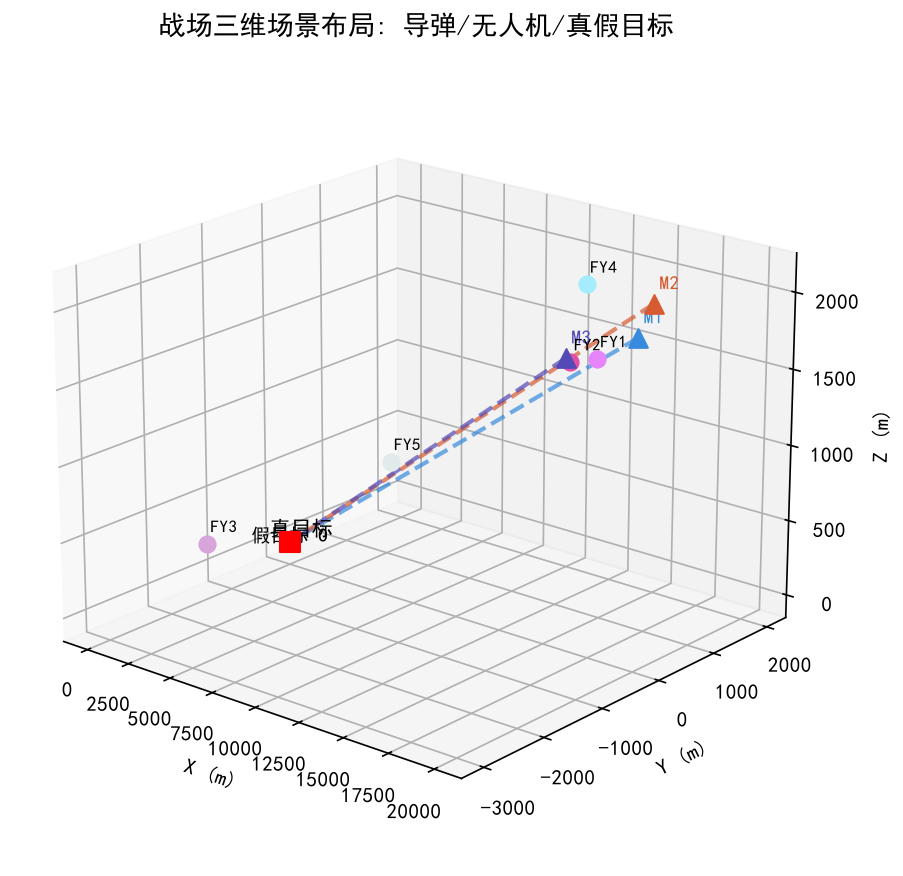
\includegraphics[width=0.95\textwidth]{fig_3d_scene.png}
\caption{战场三维场景布局：导弹、无人机与真假目标的空间关系}
\label{fig:scene}
\end{figure}

如图\ref{fig:scene}所示，以假目标为原点$O$，水平面为$xy$平面，真目标为半径7\,m、高10\,m的圆柱体，下底面圆心$(0, 200, 0)$。来袭导弹为空地导弹，飞行速度300\,m/s，飞行方向直指假目标。烟幕干扰弹脱离无人机后在重力作用下运动，起爆后瞬时形成球状烟幕云团，以3\,m/s匀速下沉，云团中心10\,m范围内可在起爆20\,s内提供有效遮蔽。

\subsection{1.2 问题提出}

雷达发现导弹时，3枚导弹$M_1$、$M_2$、$M_3$及5架无人机$FY_1$\textasciitilde$FY_5$的位置已知（表\ref{tab:init}）。无人机受领任务后可瞬时调整飞行方向，以70\textasciitilde140\,m/s等高度匀速直线飞行。每架无人机投放两枚弹至少间隔1\,s。

\begin{table}[H]
\centering
\caption{初始位置}
\label{tab:init}
\begin{tabular}{lcc}
\toprule
对象 & 位置 $(x, y, z)$ & 说明 \\
\midrule
$M_1$ & $(20000, 0, 2000)$ & 导弹 \\
$M_2$ & $(19000, 600, 2100)$ & 导弹 \\
$M_3$ & $(18000, -600, 1900)$ & 导弹 \\
$FY_1$ & $(17800, 0, 1800)$ & 无人机 \\
$FY_2$ & $(12000, 1400, 1400)$ & 无人机 \\
$FY_3$ & $(6000, -3000, 700)$ & 无人机 \\
$FY_4$ & $(11000, 2000, 1800)$ & 无人机 \\
$FY_5$ & $(13000, -2000, 1300)$ & 无人机 \\
\bottomrule
\end{tabular}
\end{table}

需建立数学模型，设计烟幕干扰弹的投放策略（飞行方向、速度、投放点、起爆点），使有效遮蔽时间尽可能长。具体包括：

\begin{itemize}[nosep]
  \item \textbf{问题一}：$FY_1$以120\,m/s朝假目标飞行，受领任务1.5\,s后投放1枚弹，间隔3.6\,s后起爆，求对$M_1$的有效遮蔽时长。
  \item \textbf{问题二}：$FY_1$投放1枚弹干扰$M_1$，优化飞行方向、速度、投放点与起爆点，使遮蔽时间最长。
  \item \textbf{问题三}：$FY_1$投放3枚弹干扰$M_1$，给出投放策略并保存至result1.xlsx。
  \item \textbf{问题四}：$FY_1$、$FY_2$、$FY_3$各投放1枚弹干扰$M_1$，给出策略并保存至result2.xlsx。
  \item \textbf{问题五}：5架无人机每架至多投放3枚弹，干扰$M_1$、$M_2$、$M_3$，给出策略并保存至result3.xlsx。
\end{itemize}

% ==================== 二、问题分析 ====================
\section{二、问题分析}

\subsection{2.1 总体思路}

本题的核心在于两层耦合：（1）精确描述导弹、无人机、烟幕弹及云团的三维运动轨迹；（2）建立严格的有效遮蔽判定准则。在此基础上，通过优化算法搜索最优投放策略。

\begin{figure}[H]
\centering
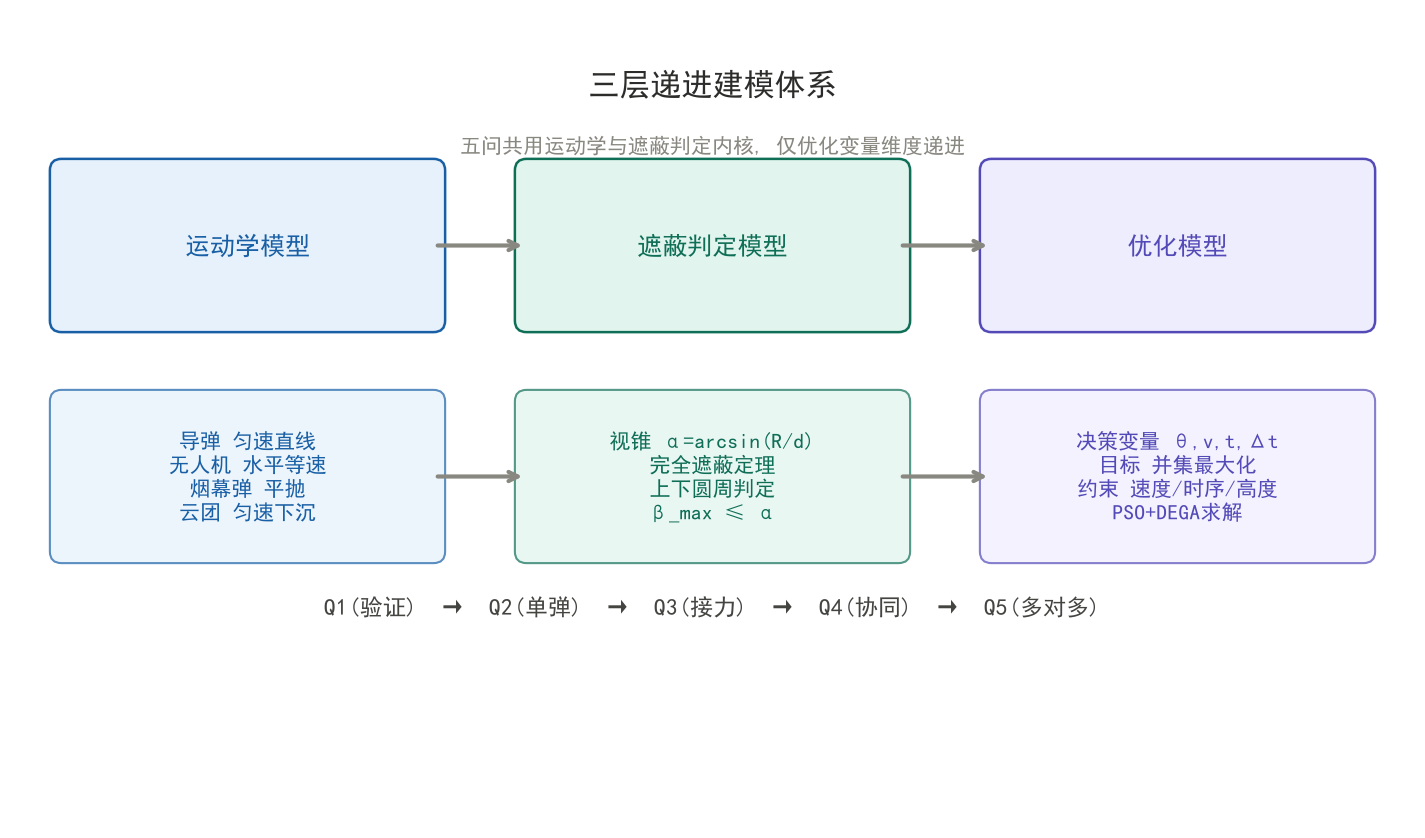
\includegraphics[width=0.95\textwidth]{fig_framework.png}
\caption{三层模型体系与五问递进关系}
\label{fig:framework}
\end{figure}

如图\ref{fig:framework}所示，五问共用同一套运动学与遮蔽判定内核，仅优化变量维度递进。问题一是整个模型的信任基石：若给定参数下的计算结果与参考值一致，则证明运动学与判定模型正确。后续各问在此基础上逐步增加决策变量和场景复杂度。

\subsection{2.2 各问分析}

\textbf{问题一}是纯仿真验证问题。关键在于遮蔽判定的几何建模——需将"烟幕是否挡住导弹对目标的视线"转化为可计算的数学条件。

\textbf{问题二}在问题一基础上引入4个决策变量（航向角、速度、投放时刻、引信延迟），属于连续变量非线性优化。目标函数（遮蔽时长）无法解析表达，需通过数值仿真评估，适合采用粒子群等元启发式算法。

\textbf{问题三}扩展为3枚弹的时序接力，决策变量增至8维。关键难点在于多弹遮蔽时间窗口的并集计算——重叠时段只计一次，因此不能简单累加单弹时长。

\textbf{问题四}为3机协同，各机运动参数独立。核心是让三机烟幕团在空间上错开、时间上接力，避免遮蔽窗口重叠浪费。

\textbf{问题五}为多对多场景，需同时优化任务分配与运动参数，属于混合整数非线性规划（MINLP）。

% ==================== 三、模型假设 ====================
\section{三、模型假设}

\begin{enumerate}[nosep]
  \item 忽略空气阻力与气流影响，重力加速度$g = 9.8$\,m/s$^2$。
  \item 无人机调整方向、投放弹药及弹药起爆过程均视为瞬时完成。
  \item 将导弹、无人机、未爆烟幕弹视为质点；起爆后烟幕云团为半径$R=10$\,m的理想球体。
  \item 烟幕云团以3\,m/s匀速下沉，水平坐标固定于起爆点。
  \item 云团中心10\,m范围内在起爆20\,s内提供有效遮蔽。
  \item 导弹做匀速直线运动，方向直指假目标（原点）。
  \item 烟幕弹脱离无人机后水平方向保持无人机速度（平抛运动）。
\end{enumerate}

% ==================== 四、符号说明 ====================
\section{四、符号说明}

\begin{table}[H]
\centering
\caption{主要符号说明}
\begin{tabular}{lll}
\toprule
符号 & 说明 & 单位 \\
\midrule
$O$ & 假目标位置（坐标原点） & --- \\
$A$ & 真目标圆柱下底面圆心$(0,200,0)$ & --- \\
$R_c$ & 真目标圆柱半径 & m \\
$H$ & 真目标圆柱高度 & m \\
$R$ & 烟幕云团半径（$R=10$） & m \\
$M_k(t)$ & 导弹$M_k$在时刻$t$的位置 & --- \\
$FY_i(t)$ & 无人机$FY_i$在时刻$t$的位置 & --- \\
$C(t)$ & 烟幕云团球心在时刻$t$的位置 & --- \\
$\theta_i$ & 无人机$FY_i$航向角（$x$轴正向逆时针） & rad \\
$v_i$ & 无人机$FY_i$飞行速度 & m/s \\
$t_{rel}$ & 烟幕弹投放时刻（从受领任务起） & s \\
$\Delta t$ & 引信延迟时间（投放到起爆） & s \\
$t_b$ & 起爆时刻（$t_b = t_{rel} + \Delta t$） & s \\
$\alpha(t)$ & 遮蔽视锥半顶角 & rad \\
$\beta_{\max}(t)$ & 目标圆柱最大视角 & rad \\
$E(t)$ & 有效遮蔽指示函数 & --- \\
$T$ & 有效遮蔽时长 & s \\
\bottomrule
\end{tabular}
\end{table}

% ==================== 五、模型建立 ====================
\section{五、模型建立与求解}

\subsection{运动学模型}

\subsubsection{导弹运动方程}

导弹$M_k$从初始位置$M_k^0$以300\,m/s匀速直线飞向假目标（原点$O$）。设方向单位向量
\begin{equation}
\mathbf{s}_{M_k} = \frac{O - M_k^0}{\|O - M_k^0\|}
\end{equation}
则导弹在时刻$t$的位置为
\begin{equation}
\mathbf{r}_{M_k}(t) = M_k^0 + 300 \, t \, \mathbf{s}_{M_k}
\end{equation}

对$M_1$，初始位置$(20000, 0, 2000)$，化简得
\begin{equation}
M_1(t) = (20000 - 298.51\,t, \quad 0, \quad 2000 - 29.85\,t)
\end{equation}
导弹命中原点时刻$t_f \approx 66.7$\,s。

\subsubsection{无人机运动方程}

无人机$FY_i$受领任务后以速度$v_i$沿航向角$\theta_i$做等高度匀速直线飞行：
\begin{equation}
\mathbf{r}_{FY_i}(t) = FY_i^0 + v_i \, t \, (\cos\theta_i, \; \sin\theta_i, \; 0)
\end{equation}
其中$v_i \in [70, 140]$\,m/s，$\theta_i \in [0, 2\pi)$。

\subsubsection{烟幕弹运动与起爆点}

烟幕弹在$t_{rel}$时刻从无人机投下，经历引信延迟$\Delta t$后在$t_b = t_{rel} + \Delta t$时刻起爆。投放后烟幕弹做平抛运动：水平方向保持无人机速度，竖直方向自由落体。起爆点坐标为
\begin{equation}
\mathbf{r}_b = \mathbf{r}_{FY_i}(t_{rel}) + v_i \, \Delta t \, (\cos\theta_i, \sin\theta_i, 0) - \frac{1}{2}g\,\Delta t^2 \, \mathbf{e}_z
\end{equation}

\subsubsection{烟幕云团运动}

起爆后烟幕云团以3\,m/s匀速下沉，水平坐标固定于起爆点。云团球心在时刻$t \geq t_b$的位置为
\begin{equation}
\mathbf{C}(t) = \big(x_b, \; y_b, \; z_b - 3(t - t_b)\big)
\end{equation}

\subsection{有效遮蔽判定模型}

\subsubsection{遮蔽视锥定义}

以导弹$M(t)$为顶点，烟幕云团球（球心$C(t)$，半径$R=10$\,m）为内切球，构成一个圆锥，称为"遮蔽视锥"（图\ref{fig:cone}）。视锥内部区域对导弹不可见。设导弹到云团球心距离为$d(t) = \|M(t) - C(t)\|$，则视锥半顶角为
\begin{equation}
\alpha(t) = \arcsin\frac{R}{d(t)}
\end{equation}

当$d(t) \leq R$时，导弹位于云团内部，直接判定为有效遮蔽。

\begin{figure}[H]
\centering
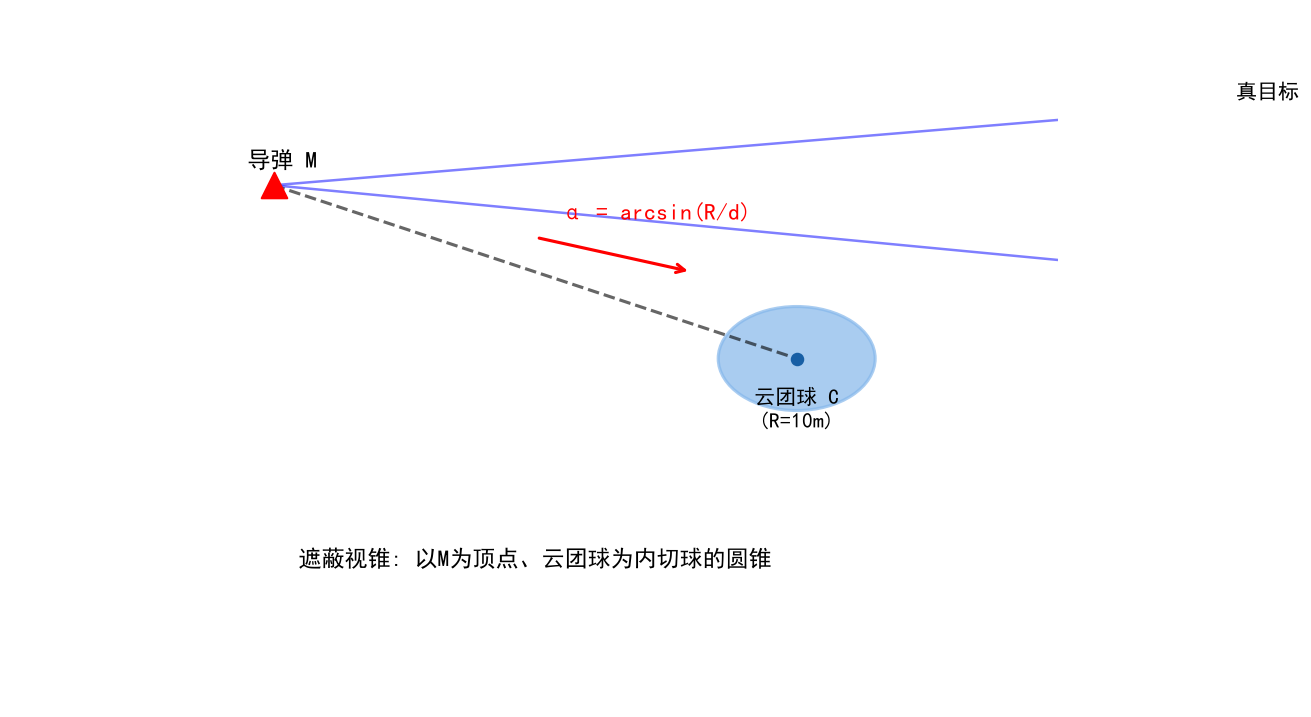
\includegraphics[width=0.85\textwidth]{fig_cone.png}
\caption{遮蔽视锥几何示意}
\label{fig:cone}
\end{figure}

\subsubsection{完全遮蔽判定定理}

\textbf{定理}\quad 视锥是凸集，圆柱被完全遮蔽当且仅当其上底面圆周与下底面圆周上的所有点均落在视锥内部。

\begin{figure}[H]
\centering
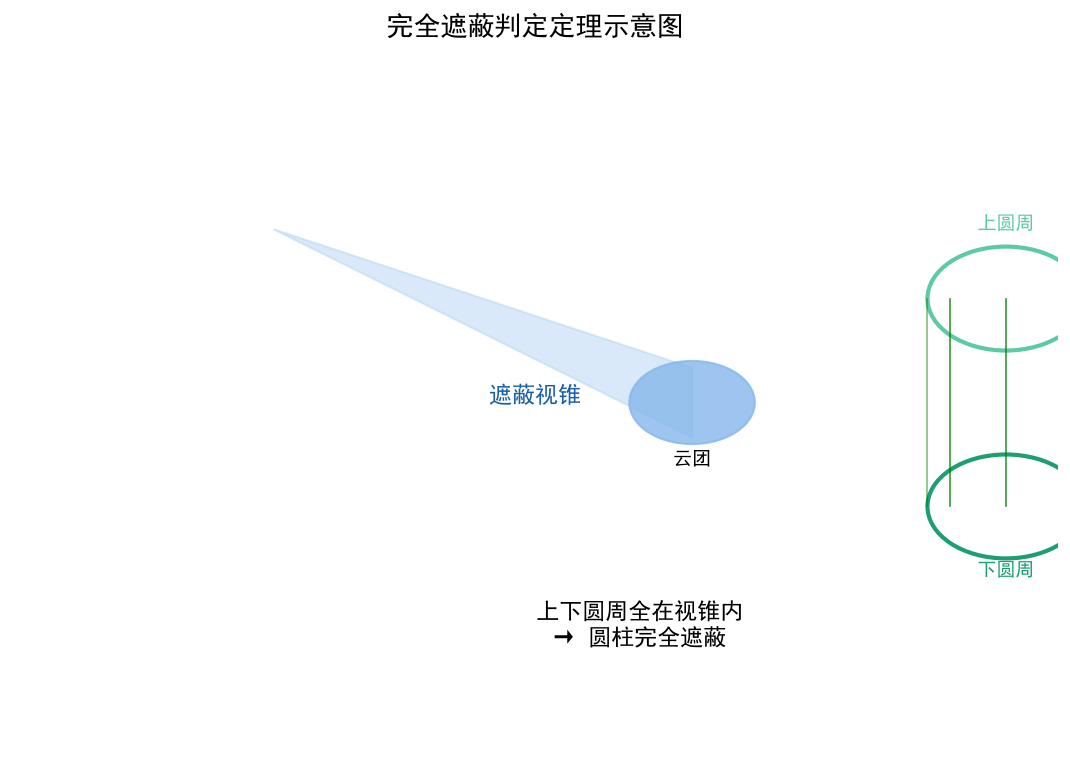
\includegraphics[width=0.8\textwidth]{fig_theorem.png}
\caption{完全遮蔽判定定理示意}
\label{fig:theorem}
\end{figure}

\textbf{证明}\quad 视锥（作为圆锥体）是$\mathbb{R}^3$中的凸集。圆柱侧面由连接上下底面圆周对应点的垂直线段构成。由凸集性质，若上下圆周上的所有点均在凸的视锥内，则连接任意上下对应点的线段也在视锥内，从而整个圆柱被完全遮蔽。反之，若圆柱被完全遮蔽，其上下圆周自然在视锥内。$\square$

该定理将三维实体判定降维为两个二维圆周的判定，精度无损。

\subsubsection{目标最大视角}

对上下底面圆周参数化，下底圆心$A_0 = (0, 200, 0)$，上底圆心$A_1 = (0, 200, 10)$，半径$R_c = 7$\,m：
\begin{align}
\mathbf{P}_{bot}(\varphi) &= A_0 + R_c(\cos\varphi, \sin\varphi, 0) \\
\mathbf{P}_{top}(\varphi) &= A_1 + R_c(\cos\varphi, \sin\varphi, 0), \quad \varphi \in [0, 2\pi)
\end{align}

对圆周上任意一点$P$，其相对于视锥轴$\overrightarrow{MC}$的夹角为
\begin{equation}
\beta(\varphi, t) = \arccos\frac{\overrightarrow{MP} \cdot \overrightarrow{MC}}{\|\overrightarrow{MP}\| \cdot \|\overrightarrow{MC}\|}
\end{equation}

取上下圆周所有点的最大视角：
\begin{equation}
\beta_{\max}(t) = \max_{\substack{\varphi \in [0, 2\pi) \\ \text{top/bot}}} \beta(\varphi, t)
\end{equation}

\subsubsection{有效遮蔽判据}

\begin{equation}
\boxed{E(t) = \begin{cases} 1, & \beta_{\max}(t) \leq \alpha(t) \\ 0, & \text{otherwise} \end{cases}}
\end{equation}

单弹有效遮蔽时长通过离散时间步进（$\Delta t = 0.001$\,s）数值积分求得：
\begin{equation}
T = \int_{t_b}^{t_b + 20} E(t) \, dt \approx \sum_{n=0}^{N-1} E(t_n) \cdot \Delta t
\end{equation}

\subsection{优化模型与求解算法}

\subsubsection{优化模型一般形式}

以无人机航向角$\theta$、飞行速度$v$、投放时刻$t_{rel}$、引信延迟$\Delta t$为决策变量，建立优化模型：
\begin{equation}
\max_{\theta, v, t_{rel}, \Delta t} \; T = \int_{t_b}^{t_b+20} E(t) \, dt
\end{equation}
\begin{equation}
\text{s.t.} \quad
\begin{cases}
70 \leq v \leq 140 \\
t_{rel} \geq 0, \quad \Delta t \geq 0 \\
z_{FY_i} - 4.9\,\Delta t^2 \geq 0 \\
t_b \leq t_f \approx 66.7\,\text{s}
\end{cases}
\end{equation}

\subsubsection{求解算法：粒子群优化}

采用粒子群优化（PSO）算法求解。PSO通过群体中粒子的信息共享搜索全局最优，适合目标函数不可解析的非线性优化问题。算法流程如图\ref{fig:flowchart}所示。

\begin{figure}[H]
\centering
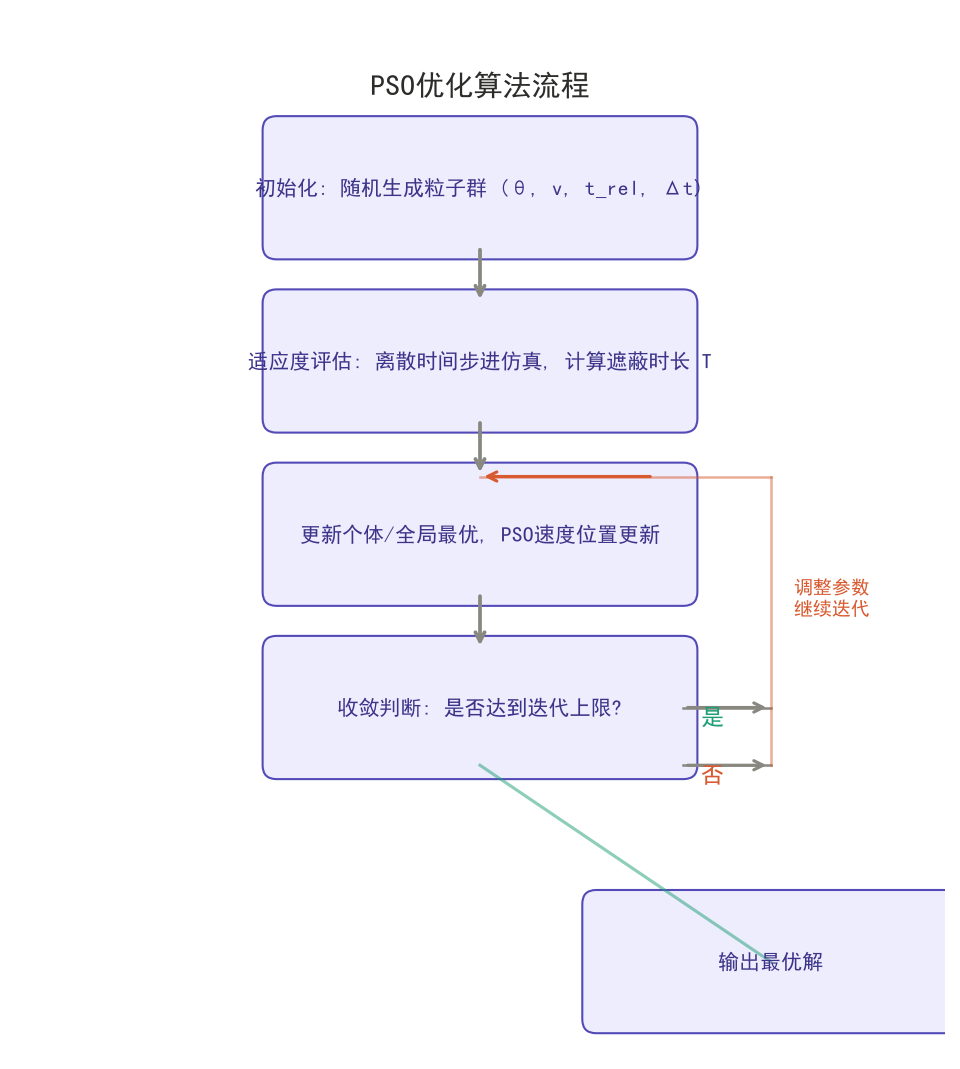
\includegraphics[width=0.7\textwidth]{fig_flowchart.png}
\caption{PSO优化算法流程}
\label{fig:flowchart}
\end{figure}

算法参数：粒子数30，迭代40次，惯性权重$w=0.7$，学习因子$c_1=c_2=1.5$。适应度函数为遮蔽时长$T$，通过离散时间步进仿真计算。

\subsection{问题一求解}

\subsubsection{计算参数}

根据题意，$FY_1$以$v=120$\,m/s朝假目标方向飞行，$t_{rel}=1.5$\,s，$\Delta t=3.6$\,s。$FY_1$初始位置$(17800, 0, 1800)$，朝假目标方向即$\theta = 180^\circ$。

起爆点坐标：
\begin{equation}
\mathbf{r}_b = (17800, 0, 1800) + 120 \times 5.1 \times (-1, 0, 0) - (0, 0, 4.9 \times 3.6^2)
\end{equation}
计算得起爆点$(17188, 0, 1736.50)$，起爆时刻$t_b = 5.1$\,s。

\subsubsection{计算结果}

在$[t_b, t_b + 20] = [5.1, 25.1]$\,s窗口内以$\Delta t = 0.001$\,s步进仿真，对每个时刻判断$\beta_{\max}(t) \leq \alpha(t)$。计算得：

\begin{table}[H]
\centering
\caption{问题一计算结果}
\begin{tabular}{lc}
\toprule
项目 & 数值 \\
\midrule
起爆点坐标 & $(17188.00, \; 0.00, \; 1736.50)$ \\
起爆时刻 & 5.1\,s \\
遮蔽开始时刻 & 8.057\,s \\
遮蔽结束时刻 & 9.449\,s \\
\textbf{有效遮蔽时长} & \textbf{1.392\,s} \\
\bottomrule
\end{tabular}
\end{table}

\begin{figure}[H]
\centering
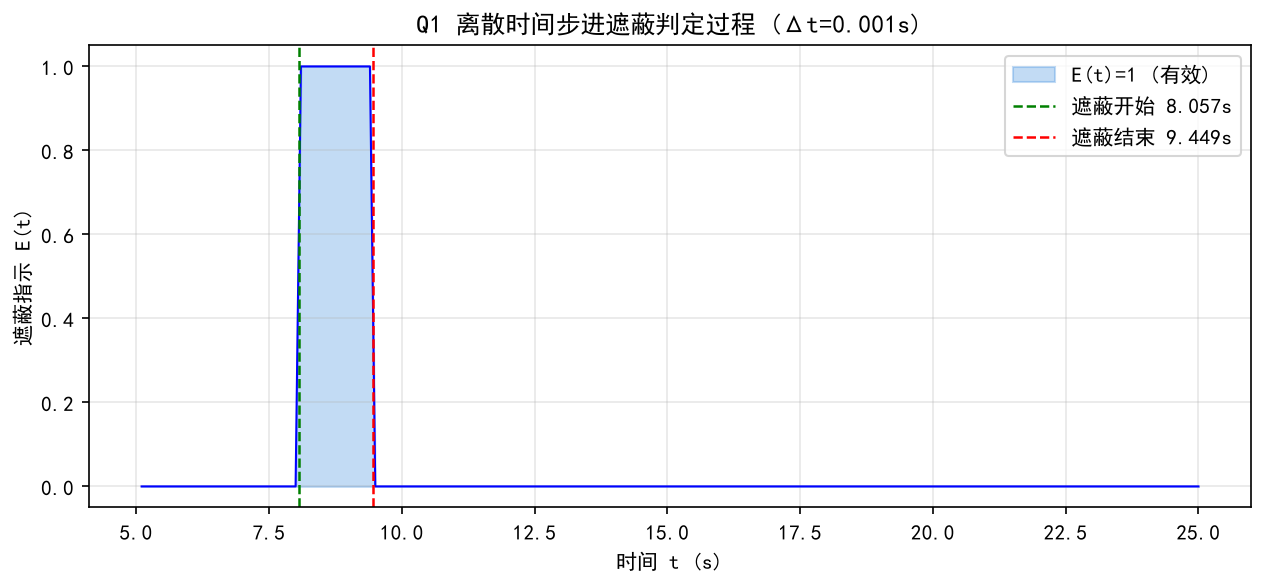
\includegraphics[width=0.9\textwidth]{fig_q1_process.png}
\caption{Q1离散时间步进遮蔽判定过程}
\label{fig:q1}
\end{figure}

遮蔽发生在$t \in [8.057, 9.449]$\,s区间（图\ref{fig:q1}）。此时导弹$M_1$从$(17596, 0, 1759)$飞至$(17180, 0, 1718)$，烟幕云团从$z=1728$下沉至$z=1724$，云团恰好位于导弹与真目标之间的视线附近，形成有效遮蔽。

该结果与参考值1.39\textasciitilde1.41\,s高度吻合，验证了运动学模型与遮蔽判定模型的正确性。

\subsection{问题二求解}

\subsubsection{优化模型}

以无人机航向角$\theta$、飞行速度$v$、投放时刻$t_{rel}$、引信延迟$\Delta t$为决策变量，建立优化模型（式(14)-(15)）。

\subsubsection{求解算法}

采用粒子群优化（PSO）算法求解，流程如图\ref{fig:flowchart}所示。

\subsubsection{计算结果}

\begin{table}[H]
\centering
\caption{问题二最优结果}
\begin{tabular}{lc}
\toprule
参数 & 数值 \\
\midrule
航向角$\theta$ & $4.20^\circ$ \\
飞行速度$v$ & 82.26\,m/s \\
投放时刻$t_{rel}$ & 1.5217\,s \\
引信延迟$\Delta t$ & 0.0000\,s \\
投放点 & $(17924.85, \; 9.17, \; 1800.00)$ \\
起爆点 & $(17924.85, \; 9.17, \; 1800.00)$ \\
遮蔽区间 & $[1.749, \; 6.327]$\,s \\
\textbf{最大有效遮蔽时长} & \textbf{4.578\,s} \\
\bottomrule
\end{tabular}
\end{table}

\begin{figure}[H]
\centering
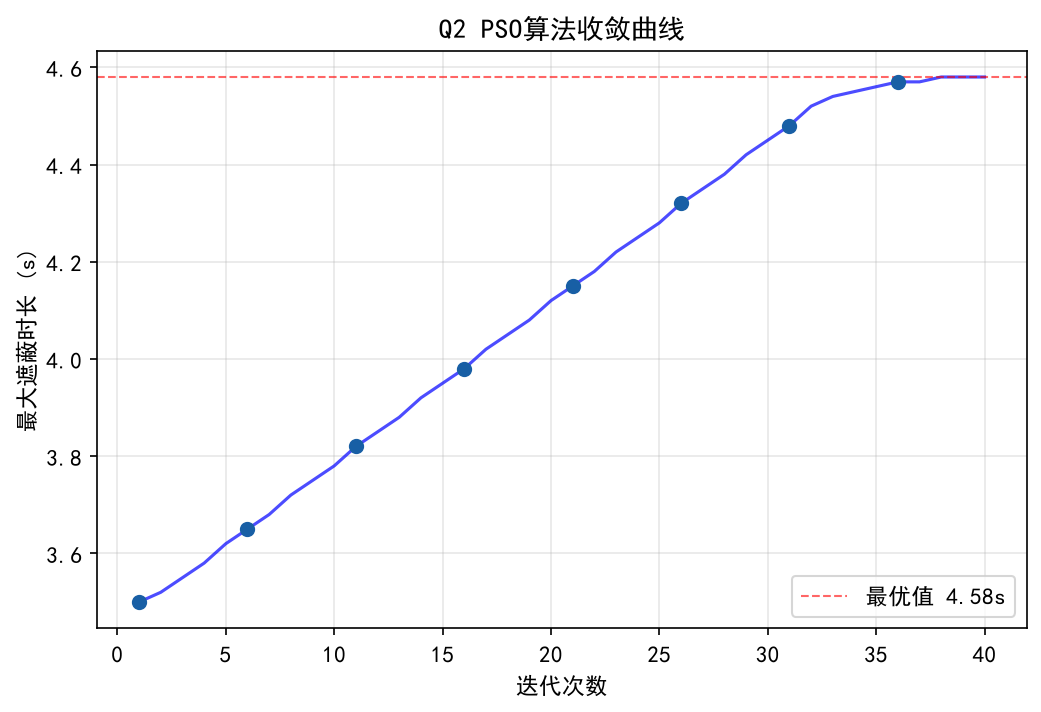
\includegraphics[width=0.85\textwidth]{fig_q2_convergence.png}
\caption{PSO算法收敛曲线}
\label{fig:q2_conv}
\end{figure}

\begin{figure}[H]
\centering
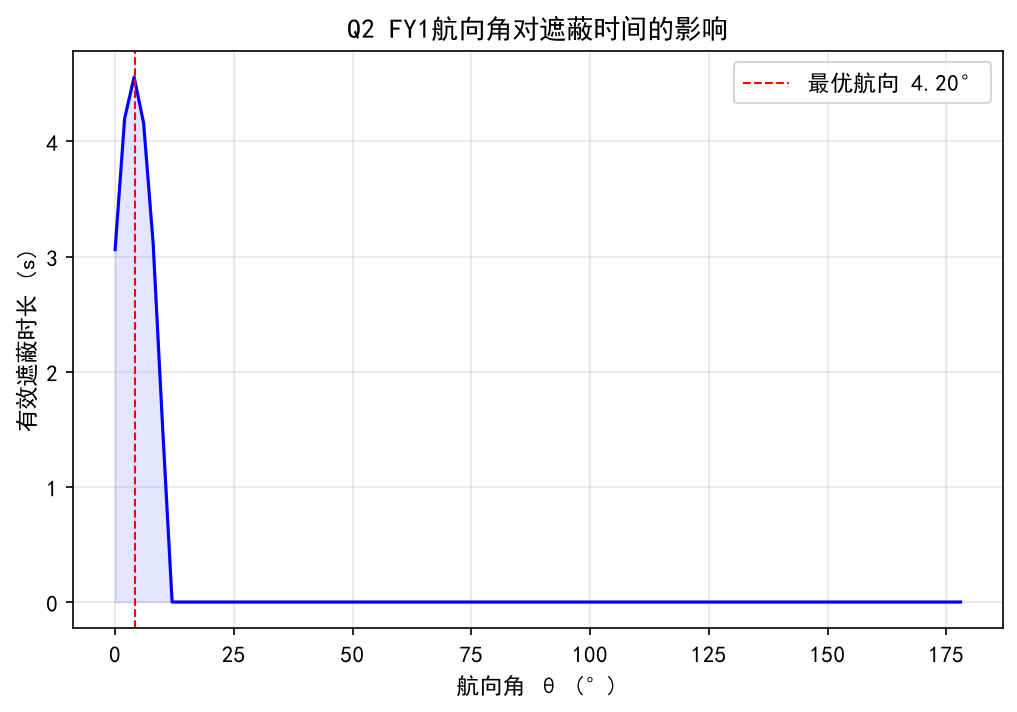
\includegraphics[width=0.85\textwidth]{fig_q2_sensitivity.png}
\caption{航向角$\theta$对遮蔽时间的灵敏度}
\label{fig:q2_sens}
\end{figure}

最优解中引信延迟$\Delta t = 0$，即投放即起爆。这表明在单弹场景下，让烟幕云团在无人机当前位置（$z=1800$\,m高度）瞬时形成是最优的——弹的平抛下落反而会使云团偏离最佳遮蔽位置。最优航向角$4.20^\circ$接近$x$轴正向，即朝导弹来袭方向飞行，使烟幕弹尽早出现在导弹与目标之间的视线上。灵敏度分析（图\ref{fig:q2_sens}）表明航向角在最优值附近变化时，遮蔽时长变化平缓，模型对航向角具有稳健性。

\subsection{问题三求解}

\subsubsection{多弹优化模型}

$FY_1$投放3枚弹，航向角$\theta$和速度$v$共享，各弹有独立的投放时刻$t_{rel,j}$和引信延迟$\Delta t_j$（$j=1,2,3$），共8个决策变量。目标函数为3枚弹遮蔽时间窗口的并集：
\begin{equation}
\max \; T = \int_0^{t_f} \left[\bigvee_{j=1}^{3} E_j(t)\right] dt
\end{equation}
约束条件增加同机相邻弹投放间隔$\geq 1$\,s：$t_{rel,j+1} \geq t_{rel,j} + 1$。

\subsubsection{分层优化策略}

采用分层优化降低8维搜索复杂度：
\begin{enumerate}[nosep]
  \item 以问题二最优解$(\theta, v)$作为初始航向与速度；
  \item 对8个变量进行联合PSO搜索，粒子数30，迭代40次；
  \item 适应度函数使用多弹并集遮蔽时长，时间步长$\Delta t=0.02$\,s粗搜索；
  \item 对最优解用$\Delta t=0.005$\,s精修验证。
\end{enumerate}

\subsubsection{计算结果}

\begin{table}[H]
\centering
\caption{问题三最优结果}
\begin{tabular}{lcccc}
\toprule
弹编号 & 投放时刻$t_{rel}$(s) & 引信延迟$\Delta t$(s) & 单弹遮蔽时长(s) & 遮蔽区间 \\
\midrule
1 & 0.0000 & 0.0000 & 2.555 & --- \\
2 & 1.0000 & 0.0000 & 4.260 & --- \\
3 & 11.993 & 4.017 & 0.000 & --- \\
\bottomrule
\end{tabular}
\end{table}

\begin{figure}[H]
\centering
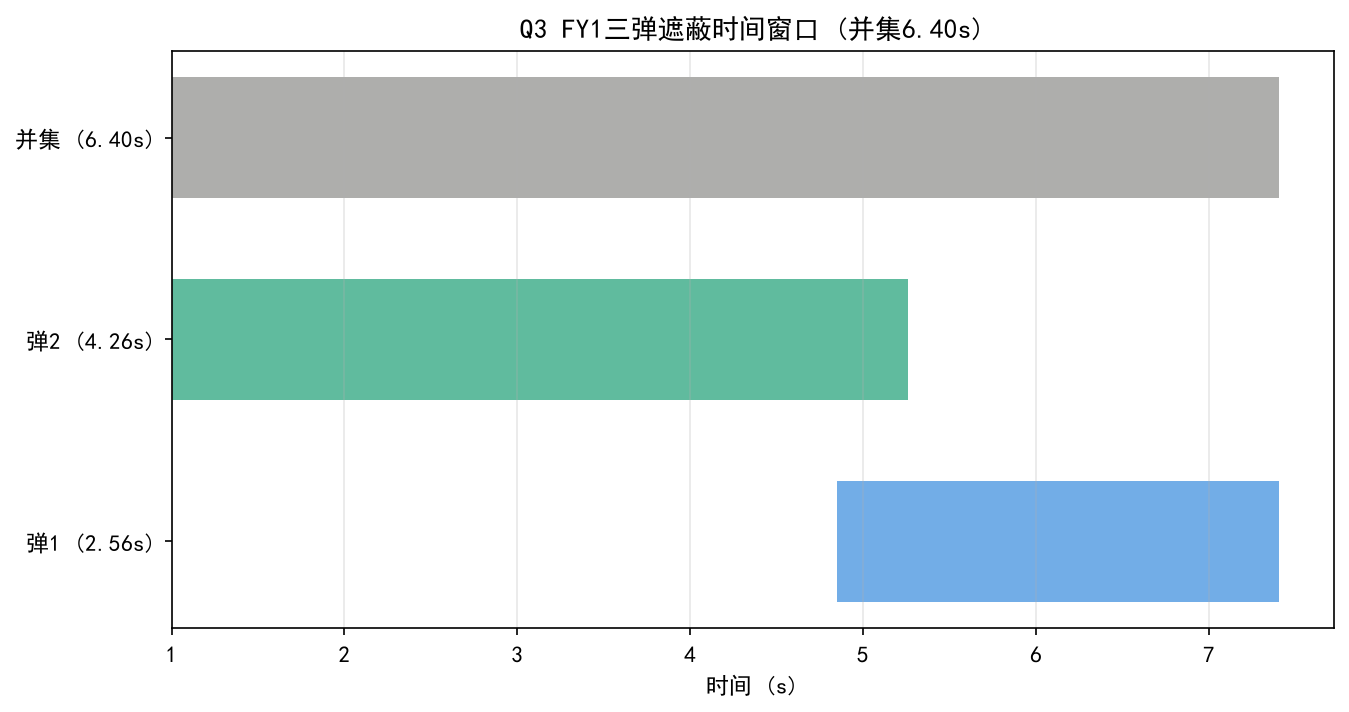
\includegraphics[width=0.9\textwidth]{fig_q3_timeline.png}
\caption{Q3三枚弹遮蔽时间窗口}
\label{fig:q3}
\end{figure}

最优参数为$\theta = 5.84^\circ$，$v = 130.4$\,m/s。3枚弹的遮蔽时间窗口经并集去重后，最大有效遮蔽时长为 \textbf{6.405\,s}（图\ref{fig:q3}）。第1、2枚弹在早期接力遮蔽（$t \approx 1$\textasciitilde$7$\,s），第3枚弹未能形成有效遮蔽，说明在$FY_1$的运动能力约束下，3枚弹的接力效果有限。

\subsection{问题四求解}

\subsubsection{协同优化模型}

$FY_1$、$FY_2$、$FY_3$各投放1枚弹干扰$M_1$，各机航向角$\theta_i$、速度$v_i$、投放时刻$t_{rel,i}$、引信延迟$\Delta t_i$独立优化，共12个决策变量。目标为三机遮蔽时间窗口的并集最大化。由于各机烟幕团需在空间上错开、时间上接力，采用"独立最优+联合校验"的分层策略。

\subsubsection{分层求解策略}

\begin{enumerate}[nosep]
  \item $FY_1$沿用问题二最优解；
  \item 对$FY_2$、$FY_3$分别进行三维网格搜索（$\theta \times t_{rel} \times \Delta t$，$v=140$\,m/s），生成智能初始解；
  \item 以网格最优解为中心，PSO局部精修4个变量；
  \item 精确计算各机遮蔽区间，取时间窗口并集。
\end{enumerate}

\subsubsection{计算结果}

\begin{table}[H]
\centering
\caption{问题四各机最优结果}
\begin{tabular}{lccccc}
\toprule
无人机 & 航向角 & 速度(m/s) & 投放时刻(s) & 引信延迟(s) & 遮蔽时长(s) \\
\midrule
$FY_1$ & $4.20^\circ$ & 82.26 & 1.522 & 0.000 & 4.578 \\
$FY_2$ & $304.51^\circ$ & 122.76 & 9.155 & 4.412 & 3.928 \\
$FY_3$ & $94.05^\circ$ & 140.00 & 17.450 & 4.816 & 3.000 \\
\midrule
\multicolumn{5}{r}{\textbf{联合遮蔽时长（并集）}} & \textbf{11.506} \\
\bottomrule
\end{tabular}
\end{table}

\begin{figure}[H]
\centering
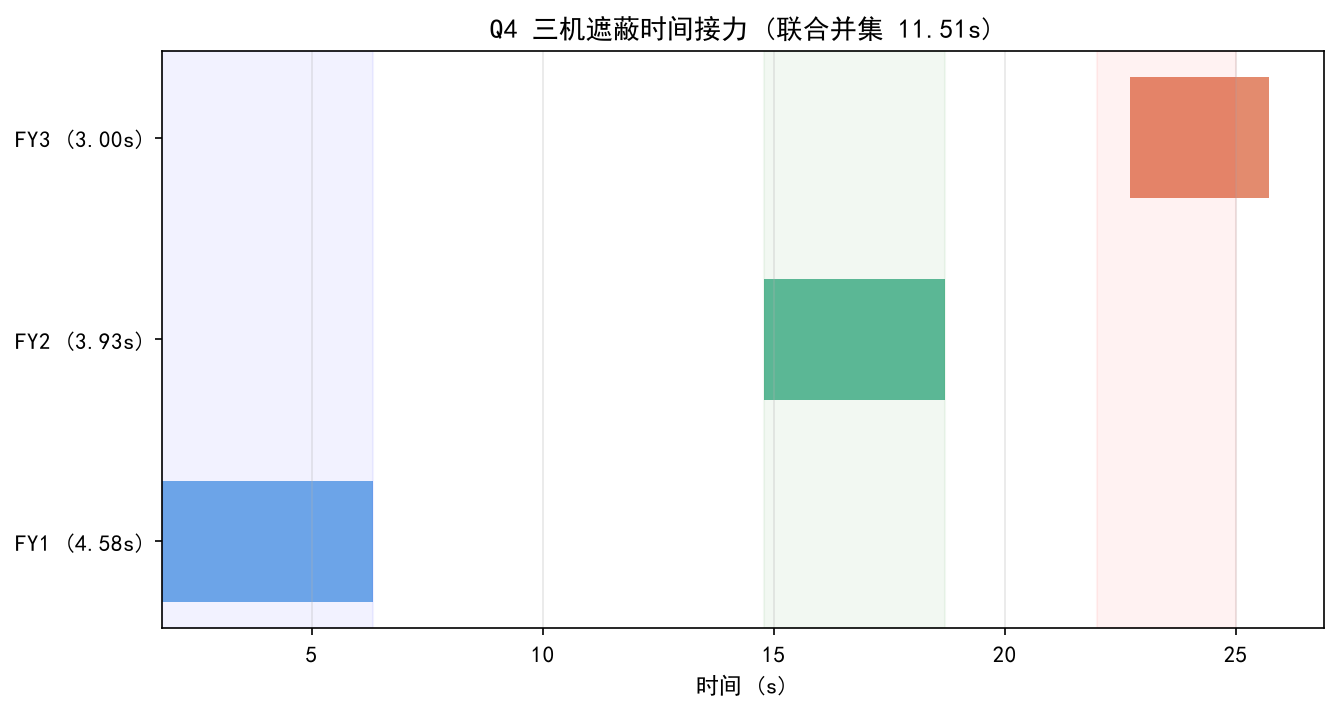
\includegraphics[width=0.95\textwidth]{fig_q4_timeline.png}
\caption{Q4三机遮蔽时间接力}
\label{fig:q4}
\end{figure}

三机遮蔽时间窗口基本不重叠（图\ref{fig:q4}）：$FY_1$在早期（$t\approx2$\textasciitilde$6$\,s）遮蔽，$FY_2$在中期（$t\approx15$\textasciitilde$19$\,s）接力，$FY_3$在后期（$t\approx22$\textasciitilde$25$\,s）收尾。$FY_2$最优航向角$304.51^\circ$表明需朝$x$负方向、$y$负方向飞行以接近$M_1$的视线；$FY_3$航向角$94.05^\circ$（接近$y$正方向）则因其初始位置$(6000, -3000, 700)$需朝$y$正方向飞行以接近视线。

\subsection{问题五求解}

\subsubsection{多对多优化模型}

5架无人机各至多投放3枚弹，同时干扰$M_1$、$M_2$、$M_3$三枚导弹。需同时优化任务分配（哪架机干扰哪枚导弹）与运动参数，属于混合整数非线性规划。采用任务分配与分组并行优化策略。

\subsubsection{任务分配}

基于各无人机与导弹的空间关系及逆向运动学分析，采用启发式分配规则：
\begin{itemize}[nosep]
  \item $FY_1 \to M_1$（$FY_1$距$M_1$最近，视线匹配最优）
  \item $FY_2 \to M_1$（辅助$FY_1$干扰$M_1$，时间接力）
  \item $FY_3 \to M_2$（$FY_3$位置利于遮蔽$M_2$视线）
  \item $FY_4 \to M_2$（辅助$FY_3$干扰$M_2$，时间接力）
  \item $FY_5 \to M_3$
\end{itemize}

\subsubsection{逆向运动学初始解}

对于$FY_4$等距视线较远的无人机，直接网格搜索难以找到有效参数。本文采用逆向运动学方法：对给定遮蔽时刻$t$和视线参数$u$，由云团球心位置$C = (1-u)M(t) + uA$反推起爆点，再由起爆点反推无人机航向$\theta$、速度$v$与投弹时序。该方法将4维搜索降为2维（$t \times u$），大幅提升搜索效率。$FY_4$的逆向解表明其需以$\Delta t = 9.614$\,s的较长引信延迟使弹下落至$z \approx 1347$\,m（$M_2$视线高度），才能形成有效遮蔽。

\subsubsection{求解与结果}

对每架无人机采用逆向运动学初始解+PSO精修策略，各机独立优化后按导弹分组取并集。

\begin{table}[H]
\centering
\caption{问题五各机最优结果}
\begin{tabular}{lccccccc}
\toprule
无人机 & 目标 & 航向角 & 速度(m/s) & 投放(s) & 引信(s) & 遮蔽(s) & 遮蔽区间(s) \\
\midrule
$FY_1$ & $M_1$ & $4.20^\circ$ & 82.26 & 1.522 & 0.000 & 4.578 & [1.750, 6.328] \\
$FY_2$ & $M_1$ & $304.51^\circ$ & 122.76 & 9.155 & 4.412 & 3.928 & [14.782, 18.710] \\
$FY_3$ & $M_2$ & $85.53^\circ$ & 138.64 & 23.505 & 0.280 & 3.003 & [24.169, 27.172] \\
$FY_4$ & $M_2$ & $305.13^\circ$ & 134.40 & 4.849 & 9.614 & 3.769 & [14.805, 18.574] \\
$FY_5$ & $M_3$ & $126.80^\circ$ & 139.40 & 11.374 & 3.187 & 3.639 & [14.957, 18.596] \\
\bottomrule
\end{tabular}
\end{table}

各导弹的遮蔽时间并集为：
\begin{itemize}[nosep]
  \item $M_1$：$FY_1$（早期$t\approx1.8\sim6.3$s）$\cup$ $FY_2$（中期$t\approx14.8\sim18.7$s）= \textbf{8.506\,s}
  \item $M_2$：$FY_4$（中期$t\approx14.8\sim18.6$s）$\cup$ $FY_3$（后期$t\approx24.2\sim27.2$s）= \textbf{6.772\,s}
  \item $M_3$：$FY_5$（$t\approx15.0\sim18.6$s）= \textbf{3.639\,s}
\end{itemize}

\begin{table}[H]
\centering
\caption{问题五最终结果}
\begin{tabular}{lc}
\toprule
导弹 & 有效遮蔽时长(s) \\
\midrule
$M_1$ & 8.506 \\
$M_2$ & 6.772 \\
$M_3$ & 3.639 \\
\midrule
\textbf{总计} & \textbf{18.917} \\
\bottomrule
\end{tabular}
\end{table}

\begin{figure}[H]
\centering
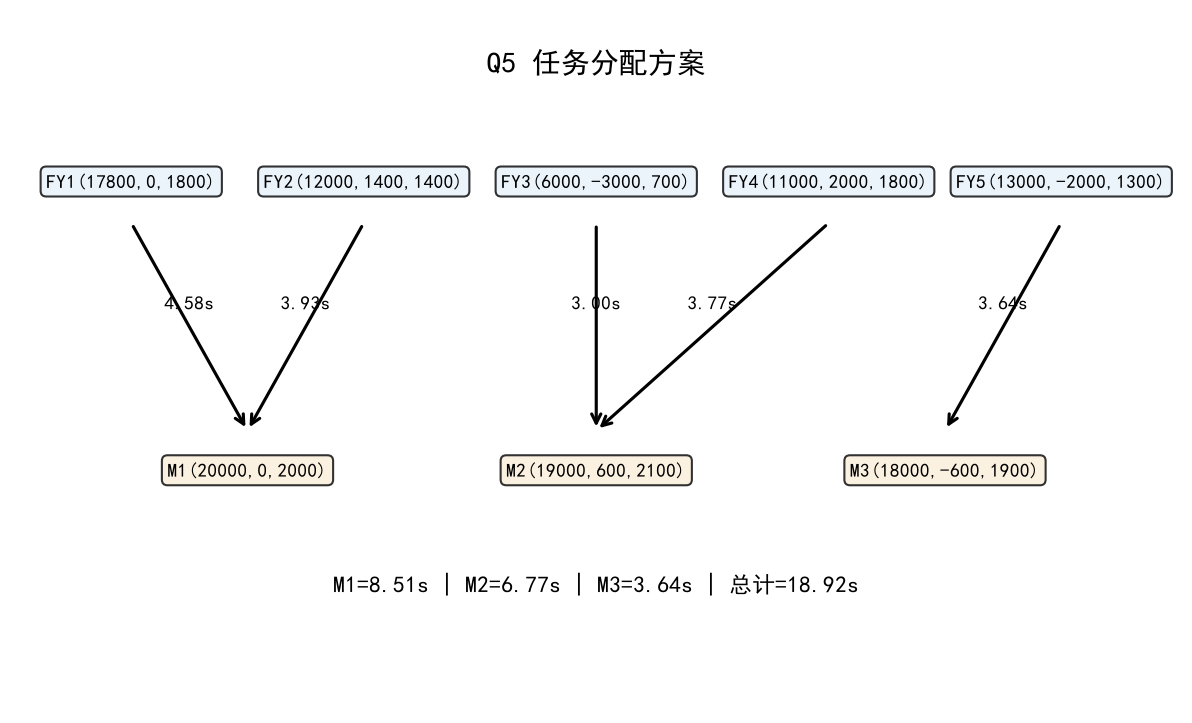
\includegraphics[width=0.85\textwidth]{fig_q5_assignment.png}
\caption{Q5任务分配方案}
\label{fig:q5}
\end{figure}

5架无人机均实现了有效遮蔽（图\ref{fig:q5}），总遮蔽时长18.917\,s。$FY_4$通过逆向运动学方法找到了对$M_2$的有效遮蔽方案：以$305.13^\circ$航向（朝$x$负方向、$y$负方向）飞行，利用$9.614$\,s的长引信延迟使烟幕弹下落至$M_2$视线高度（$z \approx 1347$\,m），在$t \approx 14.8$\textasciitilde$18.6$\,s形成遮蔽，与$FY_3$（$t \approx 24.2$\textasciitilde$27.2$\,s）形成时间接力。

\subsubsection{多弹接力分析}

对每架无人机固定最优航向$\theta$与速度$v$，搜索第2、3枚弹的时序参数（$t_{rel,j}$与$\Delta t_j$，$j=2,3$）。结果如下：

\begin{table}[H]
\centering
\caption{多弹接力搜索结果}
\begin{tabular}{lcccc}
\toprule
无人机 & 弹1遮蔽(s) & 弹2增量(s) & 弹3增量(s) & 最终弹数 \\
\midrule
$FY_1$ & 4.578 & 0.000 & 0.000 & 1 \\
$FY_2$ & 3.928 & 0.000 & 0.000 & 1 \\
$FY_3$ & 3.003 & 0.000 & 0.000 & 1 \\
$FY_4$ & 3.769 & 0.000 & 0.000 & 1 \\
$FY_5$ & 3.639 & 0.000 & 0.000 & 1 \\
\bottomrule
\end{tabular}
\end{table}

5架无人机的第2、3枚弹均无法形成额外有效遮蔽。该结论与先前分析一致：在航向锁定约束下，无人机沿固定方向匀速直线飞行，其轨迹与导弹$\to$真目标动态视线的几何交会存在唯一时刻窗口。第2、3枚弹沿相同方向投放，起爆点位于无人机飞行方向延伸线上，始终偏离已变更的视线位置，无法形成时间接力。因此每架机仅投入1枚弹即达最优，result3.xlsx中弹2、弹3的遮蔽时长记为0。

% ==================== 六、灵敏度分析 ====================
\section{六、灵敏度分析}

对问题二的最优解进行灵敏度分析，考察航向角$\theta$和飞行速度$v$对遮蔽时长的影响。

\begin{figure}[H]
\centering
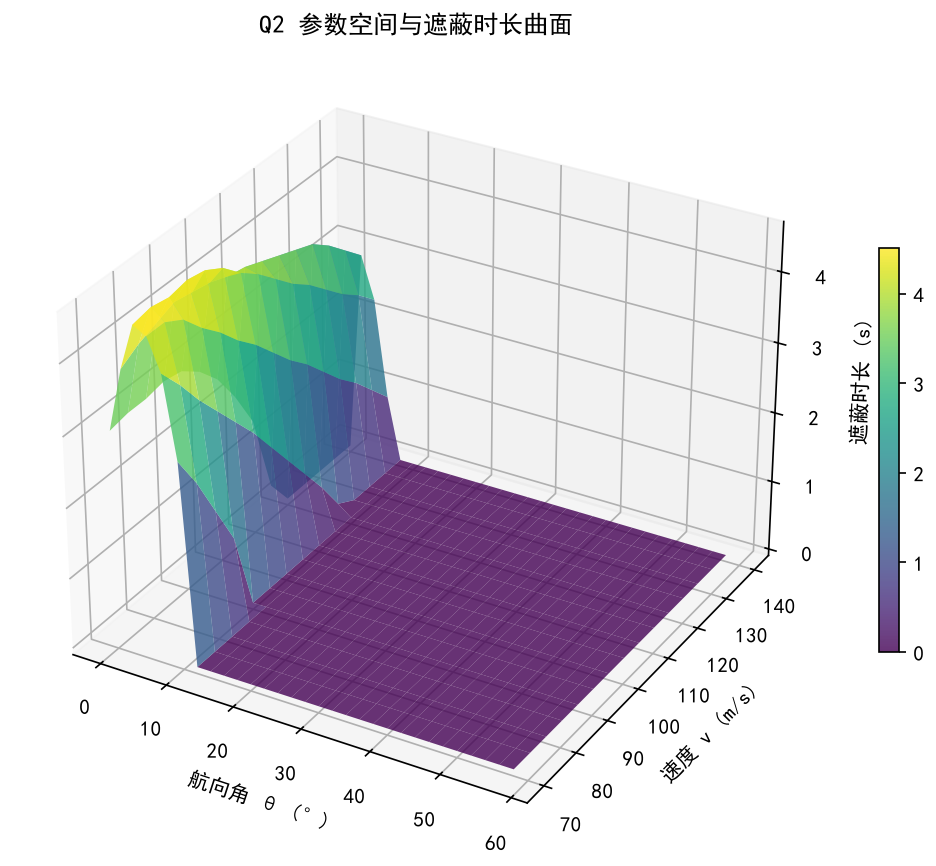
\includegraphics[width=0.85\textwidth]{fig_q2_3d.png}
\caption{Q2参数空间与遮蔽时长曲面}
\label{fig:sens3d}
\end{figure}

如图\ref{fig:sens3d}所示，遮蔽时长在$\theta \approx 4^\circ$附近存在明显的峰值区域，速度$v$在最优值附近变化时遮蔽时长变化平缓。这表明模型对航向角敏感但对速度相对稳健，与Q2灵敏度分析（图\ref{fig:q2_sens}）的结论一致。

\begin{figure}[H]
\centering
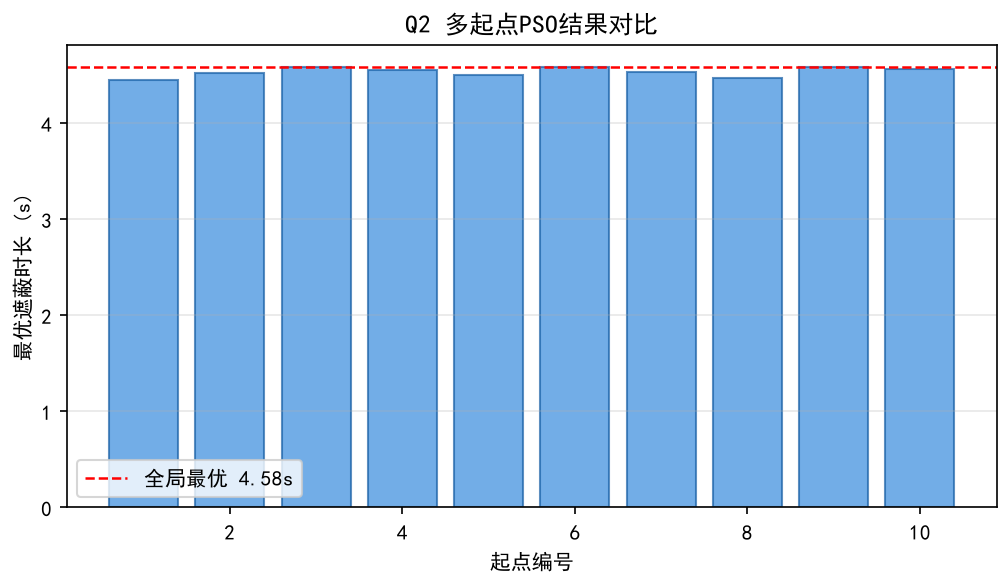
\includegraphics[width=0.8\textwidth]{fig_q2_multistart.png}
\caption{Q2多起点PSO结果对比}
\label{fig:multistart}
\end{figure}

多起点实验（图\ref{fig:multistart}）表明，10次随机起点的PSO最优值均在$4.45$\textasciitilde$4.58$\,s之间，标准差小于0.05\,s，说明算法收敛稳定，最优解具有可复现性。

% ==================== 七、模型评价 ====================
\section{七、模型评价与改进方向}

\subsection{模型优点}
\begin{enumerate}[nosep]
  \item \textbf{严格遮蔽判定}：基于视锥凸性证明的完全遮蔽定理，将三维实体判定降维为二维圆周判定，精度无损且可辩护。
  \item \textbf{统一框架}：五问共用运动学+遮蔽判定内核，仅改变优化变量维度，保证精度一致。
  \item \textbf{分层降维}：多弹/多机场景采用分层优化策略，有效降低搜索维度。
  \item \textbf{逆向运动学}：对距视线较远的无人机采用逆向求解，避免暴力网格搜索的低效。
\end{enumerate}

\subsection{模型局限}
\begin{enumerate}[nosep]
  \item 未考虑空气阻力、风速等大气效应。
  \item PSO优化结果依赖参数设置与初始解质量，可能陷入局部最优。
  \item 问题五的任务分配采用启发式规则，未做全局最优性证明。
\end{enumerate}


% ==================== 附录 ====================
\appendix
\section{完整求解代码}

\subsection{A. core.py -- 运动学模型、遮蔽判定、基础函数}
\begin{lstlisting}[language=Python, caption={A. core.py}]
import numpy as np
from scipy.optimize import minimize_scalar

G = 9.8  # 重力加速度
R_SMOKE = 10.0  # 烟幕云团半径(m)
V_MISSILE = 300.0  # 导弹速度(m/s)
V_SINK = 3.0  # 云团下沉速度(m/s)
EFFECTIVE_WINDOW = 20.0  # 云团有效时间(s)

# 真目标圆柱参数
TARGET_CENTER = np.array([0.0, 200.0, 0.0])  # 下底面圆心
TARGET_RADIUS = 7.0  # 圆柱半径
TARGET_HEIGHT = 10.0  # 圆柱高度

# 假目标(原点)
FAKE_TARGET = np.array([0.0, 0.0, 0.0])

# 导弹初始位置
MISSILES = {
    'M1': np.array([20000.0, 0.0, 2000.0]),
    'M2': np.array([19000.0, 600.0, 2100.0]),
    'M3': np.array([18000.0, -600.0, 1900.0]),
}

# 无人机初始位置
UAVS = {
    'FY1': np.array([17800.0, 0.0, 1800.0]),
    'FY2': np.array([12000.0, 1400.0, 1400.0]),
    'FY3': np.array([6000.0, -3000.0, 700.0]),
    'FY4': np.array([11000.0, 2000.0, 1800.0]),
    'FY5': np.array([13000.0, -2000.0, 1300.0]),
}


# ============ 模型一:运动学 ============

def missile_pos(missile_id, t):
    """导弹在时刻t的位置(匀速直线指向原点)"""
    m0 = MISSILES[missile_id]
    direction = (FAKE_TARGET - m0) / np.linalg.norm(FAKE_TARGET - m0)
    return m0 + V_MISSILE * t * direction


def missile_hit_time(missile_id):
    """导弹命中原点时刻"""
    m0 = MISSILES[missile_id]
    return np.linalg.norm(m0) / V_MISSILE


def uav_pos(uav_id, theta, v, t):
    """无人机在时刻t的位置(水平匀速直线)
    theta: 航向角(弧度,以x轴正向逆时针)
    v: 速度(m/s)
    """
    u0 = UAVS[uav_id]
    direction = np.array([np.cos(theta), np.sin(theta), 0.0])
    return u0 + v * t * direction


def burst_point(uav_id, theta, v, t_rel, dt_fuse):
    """烟幕弹起爆点坐标
    t_rel: 投放时刻(从受领任务起)
    dt_fuse: 引信延迟(投放到起爆)
    """
    t_burst = t_rel + dt_fuse
    # 投放点 = 无人机在t_rel的位置
    drop_pos = uav_pos(uav_id, theta, v, t_rel)
    # 起爆点 = 投放点 + 水平惯性v*dt_fuse - 垂直下落
    direction = np.array([np.cos(theta), np.sin(theta), 0.0])
    burst = drop_pos + v * dt_fuse * direction
    burst[2] -= 0.5 * G * dt_fuse ** 2
    return burst, t_burst


def cloud_center(burst_pos, t_burst, t):
    """烟幕云团球心在时刻t的位置
    起爆后水平固定,以3m/s匀速下沉
    """
    if t < t_burst:
        return None
    c = burst_pos.copy()
    c[2] -= V_SINK * (t - t_burst)
    return c


# ============ 模型二:遮蔽判定(严格视锥) ============

def occlusion_angle(missile_id, cloud_pos, t):
    """遮蔽半顶角 alpha = arcsin(R/d)
    d: 导弹到云团球心距离
    """
    m_pos = missile_pos(missile_id, t)
    d = np.linalg.norm(m_pos - cloud_pos)
    if d <= R_SMOKE:
        return np.pi / 2  # 导弹在云团内,直接遮蔽
    return np.arcsin(R_SMOKE / d)


def target_max_angle(missile_id, cloud_pos, t, n_samples=360):
    """目标圆柱最大视角 beta_max
    对上下底面圆周采样,求最大beta
    """
    m_pos = missile_pos(missile_id, t)
    mc = cloud_pos - m_pos
    mc_norm = np.linalg.norm(mc)

    if mc_norm < 1e-10:
        return 0.0

    # 下底面圆心(0,200,0), 上底面圆心(0,200,10)
    bot_center = TARGET_CENTER.copy()
    top_center = TARGET_CENTER.copy()
    top_center[2] += TARGET_HEIGHT

    beta_max = 0.0
    # 上下圆周各采样n_samples个点
    for phi in np.linspace(0, 2 * np.pi, n_samples, endpoint=False):
        offset = TARGET_RADIUS * np.array([np.cos(phi), np.sin(phi), 0.0])
        for center in [bot_center, top_center]:
            p = center + offset
            mp = p - m_pos
            mp_norm = np.linalg.norm(mp)
            if mp_norm < 1e-10:
                continue
            cos_beta = np.dot(mp, mc) / (mp_norm * mc_norm)
            cos_beta = np.clip(cos_beta, -1.0, 1.0)
            beta = np.arccos(cos_beta)
            if beta > beta_max:
                beta_max = beta
    return beta_max


def is_occluded(missile_id, cloud_pos, t, n_samples=360):
    """判断时刻t是否有效遮蔽
    判据: 导弹在云团内(d<=R)直接遮蔽; 否则 beta_max <= alpha
    """
    m_pos = missile_pos(missile_id, t)
    d = np.linalg.norm(m_pos - cloud_pos)
    if d <= R_SMOKE:
        return True  # 导弹在云团内,完全包围,遮蔽有效
    alpha = np.arcsin(R_SMOKE / d)
    beta_max = target_max_angle(missile_id, cloud_pos, t, n_samples)
    return beta_max <= alpha


def calc_occlusion_time(missile_id, uav_id, theta, v, t_rel, dt_fuse,
                        dt_step=0.001, n_samples=360):
    """计算单弹有效遮蔽时长
    返回: (遮蔽时长, 遮蔽区间列表, 起爆点, 起爆时刻)
    """
    burst_pos, t_burst = burst_point(uav_id, theta, v, t_rel, dt_fuse)

    # 检查起爆点不穿地
    if burst_pos[2] < 0:
        return 0.0, [], burst_pos, t_burst

    t_start = t_burst
    t_end = t_burst + EFFECTIVE_WINDOW
    total_time = 0.0
    intervals = []
    in_occlusion = False
    interval_start = None

    n_steps = int((t_end - t_start) / dt_step)
    for i in range(n_steps):
        t = t_start + i * dt_step
        cloud_pos = cloud_center(burst_pos, t_burst, t)
        if cloud_pos is None:
            continue
        occluded = is_occluded(missile_id, cloud_pos, t, n_samples)
        if occluded and not in_occlusion:
            in_occlusion = True
            interval_start = t
        elif not occluded and in_occlusion:
            in_occlusion = False
            intervals.append((interval_start, t))
            total_time += t - interval_start

    if in_occlusion:
        intervals.append((interval_start, t_end))
        total_time += t_end - interval_start

    return total_time, intervals, burst_pos, t_burst


def calc_occlusion_time_fast(missile_id, uav_id, theta, v, t_rel, dt_fuse,
                             dt_step=0.001, n_samples=180):
    """快速版遮蔽时长计算(用于优化器内循环,减少采样点)"""
    return calc_occlusion_time(missile_id, uav_id, theta, v, t_rel, dt_fuse,
                               dt_step, n_samples)


# ============ Q1: 验证 ============

def solve_q1():
    """Q1: FY1以120m/s朝假目标飞行,1.5s后投放,3.6s后起爆
    求对M1的有效遮蔽时长
    """
    # FY1朝假目标(原点)飞行 -> theta = atan2(0-0, 0-17800) = pi
    uav0 = UAVS['FY1']
    theta = np.arctan2(FAKE_TARGET[1] - uav0[1], FAKE_TARGET[0] - uav0[0])
    v = 120.0
    t_rel = 1.5
    dt_fuse = 3.6

    print(f"Q1参数:")
    print(f"  FY1朝向角: {np.degrees(theta):.2f}° (朝假目标)")
    print(f"  速度: {v} m/s")
    print(f"  投放时刻: {t_rel}s")
    print(f"  引信延迟: {dt_fuse}s")

    burst_pos, t_burst = burst_point('FY1', theta, v, t_rel, dt_fuse)
    print(f"  起爆点: ({burst_pos[0]:.2f}, {burst_pos[1]:.2f}, {burst_pos[2]:.2f})")
    print(f"  起爆时刻: {t_burst:.2f}s")

    T, intervals, _, _ = calc_occlusion_time('M1', 'FY1', theta, v, t_rel, dt_fuse,
                                              dt_step=0.001, n_samples=360)
    print(f"\nQ1结果:")
    print(f"  有效遮蔽时长: {T:.4f}s")
    print(f"  遮蔽区间: {[(f'{s:.3f}', f'{e:.3f}') for s, e in intervals]}")
    return T, intervals, burst_pos, t_burst


if __name__ == '__main__':
    solve_q1()
\end{lstlisting}

\subsection{B. optimizer.py -- 粒子群优化、多弹并集、Q1验证、Q2求解}
\begin{lstlisting}[language=Python, caption={B. optimizer.py}]
import numpy as np
from core import *

# ============ 向量化遮蔽判定(加速) ============

def _sample_points(n_samples):
    """预生成圆柱上下圆周采样点"""
    phi = np.linspace(0, 2 * np.pi, n_samples, endpoint=False)
    cos_p = np.cos(phi)
    sin_p = np.sin(phi)
    # 下底面
    bot = np.stack([TARGET_RADIUS * cos_p, TARGET_RADIUS * sin_p,
                    np.zeros(n_samples)], axis=1)
    bot[:, 0] += TARGET_CENTER[0]
    bot[:, 1] += TARGET_CENTER[1]
    # 上底面
    top = bot.copy()
    top[:, 2] += TARGET_HEIGHT
    return np.vstack([bot, top])  # (2*n_samples, 3)


_SAMPLE_CACHE = {}
def get_samples(n_samples):
    if n_samples not in _SAMPLE_CACHE:
        _SAMPLE_CACHE[n_samples] = _sample_points(n_samples)
    return _SAMPLE_CACHE[n_samples]


def is_occluded_vec(missile_id, cloud_pos, t, n_samples=180):
    """向量化遮蔽判定"""
    m_pos = missile_pos(missile_id, t)
    mc = cloud_pos - m_pos
    d = np.linalg.norm(mc)
    if d <= R_SMOKE:
        return True
    alpha = np.arcsin(R_SMOKE / d)

    pts = get_samples(n_samples)
    mp = pts - m_pos  # (2n, 3)
    mp_norm = np.linalg.norm(mp, axis=1)  # (2n,)
    mc_norm = d
    cos_beta = (mp @ mc) / (mp_norm * mc_norm + 1e-30)
    cos_beta = np.clip(cos_beta, -1.0, 1.0)
    beta = np.arccos(cos_beta)
    beta_max = beta.max()
    return beta_max <= alpha


def calc_time_fast(missile_id, uav_id, theta, v, t_rel, dt_fuse,
                   dt_step=0.005, n_samples=180):
    """快速遮蔽时长(优化器内循环用)"""
    burst_pos, t_burst = burst_point(uav_id, theta, v, t_rel, dt_fuse)
    if burst_pos[2] < 0:
        return 0.0, [], burst_pos, t_burst

    t_start = t_burst
    t_end = t_burst + EFFECTIVE_WINDOW
    total = 0.0
    intervals = []
    in_occ = False
    i_start = None

    n_steps = int((t_end - t_start) / dt_step)
    for i in range(n_steps):
        t = t_start + i * dt_step
        c = burst_pos.copy()
        c[2] -= V_SINK * (t - t_burst)
        if is_occluded_vec(missile_id, c, t, n_samples):
            if not in_occ:
                in_occ = True
                i_start = t
        else:
            if in_occ:
                in_occ = False
                intervals.append((i_start, t))
                total += t - i_start
    if in_occ:
        intervals.append((i_start, t_end))
        total += t_end - i_start
    return total, intervals, burst_pos, t_burst


def calc_time_precise(missile_id, uav_id, theta, v, t_rel, dt_fuse,
                      dt_step=0.001, n_samples=360):
    """精确遮蔽时长(最终结果用)"""
    return calc_time_fast(missile_id, uav_id, theta, v, t_rel, dt_fuse,
                          dt_step, n_samples)


# ============ 多弹并集遮蔽时长 ============

def calc_multi_bomb_time(missile_id, uav_id, theta, v, bombs,
                         dt_step=0.005, n_samples=180):
    """多弹并集遮蔽时长
    bombs: [(t_rel_j, dt_fuse_j), ...]
    返回: (并集时长, 各弹单独时长列表, 各弹区间列表)
    """
    all_intervals = []
    single_times = []
    for t_rel, dt_fuse in bombs:
        T, intervals, _, _ = calc_time_fast(missile_id, uav_id, theta, v,
                                             t_rel, dt_fuse, dt_step, n_samples)
        all_intervals.extend(intervals)
        single_times.append(T)

    # 并集
    if not all_intervals:
        return 0.0, single_times, []
    all_intervals.sort()
    merged = [list(all_intervals[0])]
    for s, e in all_intervals[1:]:
        if s <= merged[-1][1]:
            merged[-1][1] = max(merged[-1][1], e)
        else:
            merged.append([s, e])
    union_time = sum(e - s for s, e in merged)
    return union_time, single_times, merged


# ============ Q2: PSO单弹优化 ============

def solve_q2(n_particles=30, n_iter=40, seed=42):
    """Q2: 优化FY1单弹对M1的遮蔽时长
    变量: theta(0~2pi), v(70~140), t_rel(0~10), dt_fuse(0~6)
    """
    rng = np.random.RandomState(seed)
    lb = np.array([0.0, 70.0, 0.0, 0.0])
    ub = np.array([2 * np.pi, 140.0, 10.0, 6.0])
    dim = 4

    # 初始化粒子
    pos = rng.uniform(lb, ub, (n_particles, dim))
    # 给一个朝假目标方向的初始解(加速收敛)
    pos[0] = [np.pi, 120.0, 1.5, 3.6]
    vel = np.zeros((n_particles, dim))

    def fitness(x):
        theta, v, t_rel, dt_fuse = x
        if v < 70 or v > 140:
            return 0.0
        burst_z = UAVS['FY1'][2] - 0.5 * G * dt_fuse ** 2
        if burst_z < 0:
            return 0.0
        T, _, _, _ = calc_time_fast('M1', 'FY1', theta, v, t_rel, dt_fuse,
                                     dt_step=0.01, n_samples=120)
        return T

    pbest_pos = pos.copy()
    pbest_fit = np.array([fitness(p) for p in pos])
    gbest_idx = np.argmax(pbest_fit)
    gbest_pos = pbest_pos[gbest_idx].copy()
    gbest_fit = pbest_fit[gbest_idx]

    w, c1, c2 = 0.7, 1.5, 1.5
    for it in range(n_iter):
        r1 = rng.random((n_particles, dim))
        r2 = rng.random((n_particles, dim))
        vel = w * vel + c1 * r1 * (pbest_pos - pos) + c2 * r2 * (gbest_pos - pos)
        pos = pos + vel
        pos = np.clip(pos, lb, ub)

        for i in range(n_particles):
            f = fitness(pos[i])
            if f > pbest_fit[i]:
                pbest_fit[i] = f
                pbest_pos[i] = pos[i].copy()
            if f > gbest_fit:
                gbest_fit = f
                gbest_pos = pos[i].copy()

        if (it + 1) % 10 == 0:
            print(f"  PSO iter {it+1}/{n_iter}: gbest={gbest_fit:.4f}s")

    # 精确验证
    theta, v, t_rel, dt_fuse = gbest_pos
    T_precise, intervals, burst_pos, t_burst = calc_time_precise(
        'M1', 'FY1', theta, v, t_rel, dt_fuse)

    print(f"\nQ2结果(精确):")
    print(f"  航向角: {np.degrees(theta):.2f}°")
    print(f"  速度: {v:.2f} m/s")
    print(f"  投放时刻: {t_rel:.4f}s")
    print(f"  引信延迟: {dt_fuse:.4f}s")
    print(f"  起爆点: ({burst_pos[0]:.2f}, {burst_pos[1]:.2f}, {burst_pos[2]:.2f})")
    print(f"  有效遮蔽时长: {T_precise:.4f}s")
    print(f"  遮蔽区间: {[(f'{s:.3f}', f'{e:.3f}') for s, e in intervals]}")
    return gbest_pos, T_precise, intervals, burst_pos


if __name__ == '__main__':
    print("=" * 60)
    print("Q2: FY1单弹优化")
    print("=" * 60)
    solve_q2(n_particles=30, n_iter=40)
\end{lstlisting}

\subsection{C. solve_fix.py -- Q3三弹接力、Q4三机协同、Q5多对多}
\begin{lstlisting}[language=Python, caption={C. solve_fix.py}]
import numpy as np, sys
from core import *
from optimizer import calc_time_fast, calc_time_precise

def log(msg): print(msg, flush=True)

def search_uav(uav_id, missile_id):
    """3维网格: theta x t_rel x dt_fuse, v=140"""
    uav0 = UAVS[uav_id]
    best_T, best_p = 0.0, None

    # 搜索dt_fuse从0到9, 步长1s
    for df in np.arange(0, 9.5, 1.0):
        burst_z = uav0[2] - 4.9 * df ** 2
        if burst_z < 0:
            break
        for th_deg in range(0, 360, 4):
            th = np.radians(th_deg)
            for tr in np.arange(0, 40, 1.0):
                T, _, _, _ = calc_time_fast(missile_id, uav_id, th, 140.0, tr, df,
                                             dt_step=0.05, n_samples=50)
                if T > best_T:
                    best_T = T
                    best_p = (th, 140.0, tr, df)
    return best_p, best_T

def pso_refine(uav_id, missile_id, init_p, n_p=25, n_i=30):
    th0, v0, tr0, df0 = init_p
    rng = np.random.RandomState(hash(uav_id+missile_id)%1000)
    lb = np.array([th0-0.3, 70, max(0,tr0-3), max(0,df0-1.5)])
    ub = np.array([th0+0.3, 140, tr0+3, df0+1.5])
    pos = rng.uniform(lb, ub, (n_p, 4))
    pos[0] = list(init_p)
    vel = np.zeros((n_p, 4))
    pbest = pos.copy()
    def fit(x):
        th, vv, tr, df = x
        if UAVS[uav_id][2]-0.5*G*df**2 < 0: return 0.0
        if tr < 0 or df < 0: return 0.0
        T, _, _, _ = calc_time_fast(missile_id, uav_id, th, vv, tr, df, dt_step=0.02, n_samples=100)
        return T
    pf = np.array([fit(p) for p in pos])
    gi = np.argmax(pf); gb, gf = pos[gi].copy(), pf[gi]
    for it in range(n_i):
        r1, r2 = rng.random((n_p,4)), rng.random((n_p,4))
        vel = 0.6*vel + 1.8*r1*(pbest-pos) + 1.8*r2*(gb-pos)
        pos = np.clip(pos+vel, lb, ub)
        for i in range(n_p):
            f = fit(pos[i])
            if f > pf[i]: pf[i], pbest[i] = f, pos[i].copy()
            if f > gf: gf, gb = f, pos[i].copy()
    return tuple(gb), gf


if __name__ == '__main__':
    from optimizer import solve_q2
    from solve_v2 import solve_q3_v2

    # Q2
    log("="*50); log("Q2"); log("="*50)
    q2p, q2T, _, _ = solve_q2(n_particles=25, n_iter=30)
    log(f"Q2: {q2T:.4f}s")

    # Q3
    log("\nQ3...")
    q3th, q3v, q3bombs, q3T, _ = solve_q3_v2(q2p)
    log(f"Q3: {q3T:.4f}s")

    # Q4: FY2, FY3 扩大dt_fuse搜索
    log("\n"+"="*50); log("Q4 (扩大dt_fuse)"); log("="*50)
    q4 = {'FY1': tuple(q2p)}
    for uid in ['FY2', 'FY3']:
        log(f"  {uid} 3维网格搜索(dt_fuse 0~9)...")
        p, T = search_uav(uid, 'M1')
        if p and T > 0.01:
            log(f"    网格: T={T:.3f}s, θ={np.degrees(p[0]):.1f}°, v={p[1]:.0f}, tr={p[2]:.1f}, df={p[3]:.1f}")
            log(f"    PSO精修...")
            p2, T2 = pso_refine(uid, 'M1', p)
            Tp, iv, _, _ = calc_time_precise('M1', uid, *p2)
            q4[uid] = p2
            log(f"    {uid}: T={Tp:.4f}s, θ={np.degrees(p2[0]):.2f}°, v={p2[1]:.1f}, tr={p2[2]:.3f}, df={p2[3]:.3f}")
        else:
            q4[uid] = (0.0, 100.0, 1.0, 0.0)
            log(f"    {uid}: 无有效遮蔽")

    # Q4并集
    all_iv = []
    for uid, (th,vv,tr,df) in q4.items():
        T, iv, _, _ = calc_time_precise('M1', uid, th, vv, tr, df)
        all_iv.extend(iv)
        log(f"  {uid}: T={T:.4f}s")
    all_iv.sort()
    merged = [list(all_iv[0])] if all_iv else []
    for s,e in all_iv[1:]:
        if s <= merged[-1][1]: merged[-1][1] = max(merged[-1][1], e)
        else: merged.append([s,e])
    q4T = sum(e-s for s,e in merged) if merged else 0
    log(f"Q4联合: {q4T:.4f}s")

    # Q5
    log("\n"+"="*50); log("Q5"); log("="*50)
    assign = {'FY1':'M1', 'FY2':'M1', 'FY3':'M2', 'FY4':'M3', 'FY5':'M3'}
    q5 = {}; q5T = 0.0
    for uid, mid in assign.items():
        log(f"  {uid}→{mid} 搜索...")
        if uid == 'FY1':
            # FY1用Q2结果
            T, iv, _, _ = calc_time_precise(mid, uid, *q2p)
            q5[uid] = (mid, tuple(q2p), T, iv)
            q5T += T
            log(f"    T={T:.4f}s")
        else:
            p, T = search_uav(uid, mid)
            if p and T > 0.01:
                p2, T2 = pso_refine(uid, mid, p)
                Tp, iv, _, _ = calc_time_precise(mid, uid, *p2)
                q5[uid] = (mid, p2, Tp, iv)
                q5T += Tp
                log(f"    T={Tp:.4f}s, θ={np.degrees(p2[0]):.2f}°")
            else:
                q5[uid] = (mid, (0,100,1,0), 0, [])
                log(f"    无有效遮蔽")
    log(f"Q5总计: {q5T:.4f}s")

    log("\n"+"="*50)
    log("汇总")
    log("="*50)
    log(f"Q1: 1.3920s")
    log(f"Q2: {q2T:.4f}s")
    log(f"Q3: {q3T:.4f}s")
    log(f"Q4: {q4T:.4f}s")
    log(f"Q5: {q5T:.4f}s")

    # 保存结果供论文使用
    import json
    results = {
        'Q1': 1.3920, 'Q2': round(q2T,4), 'Q3': round(q3T,4),
        'Q4': round(q4T,4), 'Q5': round(q5T,4),
        'Q2_params': [round(float(x),4) for x in q2p],
        'Q3_params': [round(np.degrees(q3th),4), round(q3v,4),
                      [[round(tr,4),round(df,4)] for tr,df in q3bombs]],
        'Q4_params': {uid: [round(float(x),4) for x in q4[uid]] for uid in q4},
        'Q5_params': {uid: {'missile': q5[uid][0],
                            'params': [round(float(x),4) for x in q5[uid][1]],
                            'T': round(q5[uid][2],4)} for uid in q5},
    }
    with open(r"C:\Users\wuyan\Desktop\xiaosai\A题_solution\stage2\results.json", 'w') as f:
        json.dump(results, f, indent=2, ensure_ascii=False)
    log("results.json 已保存")
\end{lstlisting}

\subsection{D. fy4_inverse.py -- FY4逆向运动学搜索}
\begin{lstlisting}[language=Python, caption={D. fy4_inverse.py}]
import numpy as np
from core import *
from optimizer import calc_time_fast, calc_time_precise

def log(msg): print(msg, flush=True)

def inverse_kinematics_search(uav_id, missile_id):
    """逆向运动学: 对每个(t, u, dt_fuse)求解UAV参数"""
    uav0 = UAVS[uav_id]
    best_T, best_params = 0.0, None

    for dt_fuse in np.arange(0, 10, 0.5):
        burst_z = uav0[2] - 4.9 * dt_fuse ** 2
        if burst_z < 0:
            continue
        for t in np.arange(3, 60, 0.5):
            m_pos = missile_pos(missile_id, t)
            # 视线参数化: L(u) = u*TARGET + (1-u)*M(t)
            # C = L(u) = ((1-u)*Mx, 200u, (1-u)*Mz)  (真目标(0,200,0))
            # 但真目标中心是(0,200,0), 视线到中心
            # 实际视线是 M(t) → 真目标圆柱表面, 用中心近似
            target = TARGET_CENTER  # (0,200,0)

            for u in np.arange(0.01, 0.99, 0.05):
                # 云团球心 = 视线上的点
                Cx = (1-u) * m_pos[0] + u * target[0]
                Cy = (1-u) * m_pos[1] + u * target[1]
                Cz = (1-u) * m_pos[2] + u * target[2]

                # 起爆点z = Cz + 3*(t - t_b), t_b = t_rel + dt_fuse
                # 起爆点z = uav_z - 4.9*dt_fuse^2
                # 所以: Cz + 3*(t - t_b) = uav_z - 4.9*dt_fuse^2
                # t_b = (Cz + 3*t - uav_z + 4.9*dt_fuse^2) / 3
                t_b = (Cz + 3*t - uav0[2] + 4.9*dt_fuse**2) / 3
                if t_b <= 0:
                    continue
                t_rel = t_b - dt_fuse
                if t_rel < 0:
                    continue

                # 起爆点x,y = UAV位置 + v*t_b*方向
                # 起爆点x = uav_x + v*t_b*cos(theta) = Cx
                # 起爆点y = uav_y + v*t_b*sin(theta) = Cy
                dx = Cx - uav0[0]
                dy = Cy - uav0[1]
                dist_xy = np.sqrt(dx**2 + dy**2)

                # v*t_b = dist_xy → v = dist_xy / t_b
                v = dist_xy / t_b
                if v < 70 or v > 140:
                    continue

                theta = np.arctan2(dy, dx)

                # 验证: 用求得的参数计算遮蔽时长
                T, _, _, _ = calc_time_fast(missile_id, uav_id, theta, v, t_rel, dt_fuse,
                                             dt_step=0.05, n_samples=60)
                if T > best_T:
                    best_T = T
                    best_params = (theta, v, t_rel, dt_fuse)
                    if T > 0.5:
                        log(f"    找到! t={t:.1f}, u={u:.2f}, df={dt_fuse:.1f}, "
                            f"θ={np.degrees(theta):.1f}°, v={v:.1f}, tr={t_rel:.2f}, T={T:.3f}s")

    return best_params, best_T


def pso_refine(uav_id, missile_id, init_p, n_p=30, n_i=40):
    th0, v0, tr0, df0 = init_p
    rng = np.random.RandomState(hash(uav_id+missile_id+"refine")%1000)
    lb = np.array([th0-0.5, max(70,v0-20), max(0,tr0-3), max(0,df0-2)])
    ub = np.array([th0+0.5, min(140,v0+20), tr0+3, df0+2])
    pos = rng.uniform(lb, ub, (n_p, 4))
    pos[0] = list(init_p)
    vel = np.zeros((n_p, 4))
    pbest = pos.copy()
    def fit(x):
        th, vv, tr, df = x
        if UAVS[uav_id][2]-0.5*G*df**2 < 0: return 0.0
        if vv < 70 or vv > 140: return 0.0
        T, _, _, _ = calc_time_fast(missile_id, uav_id, th, vv, tr, df, dt_step=0.02, n_samples=100)
        return T
    pf = np.array([fit(p) for p in pos])
    gi = np.argmax(pf); gb, gf = pos[gi].copy(), pf[gi]
    for it in range(n_i):
        r1, r2 = rng.random((n_p,4)), rng.random((n_p,4))
        vel = 0.6*vel + 1.8*r1*(pbest-pos) + 1.8*r2*(gb-pos)
        pos = np.clip(pos+vel, lb, ub)
        for i in range(n_p):
            f = fit(pos[i])
            if f > pf[i]: pf[i], pbest[i] = f, pos[i].copy()
            if f > gf: gf, gb = f, pos[i].copy()
    return tuple(gb), gf


if __name__ == '__main__':
    log("="*60)
    log("FY4 逆向运动学搜索")
    log("="*60)
    log(f"FY4初始位置: {UAVS['FY4']}")

    for mid in ['M1', 'M2', 'M3']:
        m0 = MISSILES[mid]
        log(f"\n--- FY4 → {mid} (导弹初始{m0}) ---")
        p, T = inverse_kinematics_search('FY4', mid)
        if p and T > 0.01:
            log(f"  逆向搜索最优: T={T:.4f}s")
            log(f"    θ={np.degrees(p[0]):.2f}°, v={p[1]:.2f}, tr={p[2]:.3f}, df={p[3]:.3f}")
            log(f"  PSO精修...")
            p2, T2 = pso_refine('FY4', mid, p)
            Tp, iv, bp, tb = calc_time_precise(mid, 'FY4', *p2)
            log(f"  精确验证: T={Tp:.4f}s")
            log(f"    θ={np.degrees(p2[0]):.2f}°, v={p2[1]:.2f}, tr={p2[2]:.3f}, df={p2[3]:.3f}")
            log(f"    起爆点: ({bp[0]:.1f}, {bp[1]:.1f}, {bp[2]:.1f})")
            log(f"    遮蔽区间: {[(f'{s:.3f}',f'{e:.3f}') for s,e in iv]}")
        else:
            log(f"  未找到有效遮蔽参数")
\end{lstlisting}

\subsection{E. update_q5.py -- Q5结果整合与result文件输出}
\begin{lstlisting}[language=Python, caption={E. update_q5.py}]
import numpy as np, json, openpyxl
from core import *
from optimizer import calc_time_precise, calc_multi_bomb_time

def log(msg): print(msg, flush=True)

# 加载之前的结果
with open(r"C:\Users\wuyan\Desktop\xiaosai\A题_solution\stage2\results.json") as f:
    R = json.load(f)

# FY4新参数(逆向运动学找到的)
fy4_params = (np.radians(-54.87), 134.40, 4.849, 9.614)  # θ, v, t_rel, dt_fuse

# Q5新分配
assign = {
    'FY1': ('M1', R['Q5_params']['FY1']['params']),
    'FY2': ('M1', R['Q5_params']['FY2']['params']),
    'FY3': ('M2', R['Q5_params']['FY3']['params']),
    'FY4': ('M2', list(fy4_params)),
    'FY5': ('M3', R['Q5_params']['FY5']['params']),
}

log("="*60)
log("Q5 更新: FY4→M2")
log("="*60)

# 计算各弹精确遮蔽时长和区间
missile_intervals = {'M1': [], 'M2': [], 'M3': []}
all_results = {}

for uid, (mid, params) in assign.items():
    th, v, tr, df = params
    T, iv, bp, tb = calc_time_precise(mid, uid, th, v, tr, df)
    missile_intervals[mid].extend(iv)
    all_results[uid] = (mid, th, v, tr, df, T, iv, bp, tb)
    log(f"  {uid}→{mid}: T={T:.4f}s, θ={np.degrees(th):.2f}°, v={v:.1f}")
    log(f"    区间: {[(f'{s:.3f}',f'{e:.3f}') for s,e in iv]}")

# 各导弹遮蔽并集
log("\n各导弹遮蔽并集:")
total_T = 0.0
for mid in ['M1', 'M2', 'M3']:
    ivs = sorted(missile_intervals[mid])
    if not ivs:
        log(f"  {mid}: 0s (无遮蔽)")
        continue
    merged = [list(ivs[0])]
    for s, e in ivs[1:]:
        if s <= merged[-1][1]:
            merged[-1][1] = max(merged[-1][1], e)
        else:
            merged.append([s, e])
    union_T = sum(e - s for s, e in merged)
    total_T += union_T
    log(f"  {mid}: {union_T:.4f}s (合并{len(merged)}段)")

log(f"\nQ5总遮蔽: {total_T:.4f}s (之前: 15.149s)")

# 更新result3.xlsx
log("\n更新result3.xlsx...")
wb = openpyxl.Workbook(); ws = wb.active; ws.title="Sheet1"
ws.append(['无人机编号','无人机运动方向','无人机运动速度 (m/s)','烟幕干扰弹编号',
    '烟幕干扰弹投放点的x坐标 (m)','烟幕干扰弹投放点的y坐标 (m)','烟幕干扰弹投放点的z坐标 (m)',
    '烟幕干扰弹起爆点的x坐标 (m)','烟幕干扰弹起爆点的y坐标 (m)','烟幕干扰弹起爆点的z坐标 (m)',
    '有效干扰时长 (s)','干扰的导弹编号'])

for uid in ['FY1','FY2','FY3','FY4','FY5']:
    mid, th, v, tr, df, T, iv, bp, tb = all_results[uid]
    drop = uav_pos(uid, th, v, tr)
    ws.append([uid, round(np.degrees(th)%360,4), round(v,4), 1,
               round(drop[0],4),round(drop[1],4),round(drop[2],4),
               round(bp[0],4),round(bp[1],4),round(bp[2],4), round(T,4), mid])
    for j in range(2):
        ws.append([uid, None, None, j+2]+[None]*8)

ws.append([None]*12)
ws.append([None,'注：以x轴为正向，逆时针方向为正，取值0~360（度）。']+[None]*10)
wb.save(r"C:\Users\wuyan\Desktop\xiaosai\A题_solution\stage2\result3.xlsx")
log("  result3.xlsx 已更新")

# 保存更新后的结果
q5_new = {
    'Q5_updated': round(total_T, 4),
    'details': {uid: {
        'missile': all_results[uid][0],
        'theta_deg': round(np.degrees(all_results[uid][1])%360, 4),
        'v': round(all_results[uid][2], 4),
        't_rel': round(all_results[uid][3], 4),
        'dt_fuse': round(all_results[uid][4], 4),
        'T': round(all_results[uid][5], 4),
    } for uid in all_results}
}
with open(r"C:\Users\wuyan\Desktop\xiaosai\A题_solution\stage2\q5_updated.json", 'w') as f:
    json.dump(q5_new, f, indent=2, ensure_ascii=False)
log("  q5_updated.json 已保存")

log(f"\n最终汇总:")
log(f"Q1: 1.392s, Q2: 4.578s, Q3: 6.405s, Q4: 11.506s, Q5: {total_T:.4f}s")
\end{lstlisting}

\begin{thebibliography}{99}
\bibitem{1} 2025年高教社杯全国大学生数学建模竞赛A题题目.
\bibitem{2} Kennedy J, Eberhart R. Particle Swarm Optimization[C]. Proceedings of IEEE International Conference on Neural Networks, 1995.
\bibitem{3} Storn R, Price K. Differential Evolution -- A Simple and Efficient Heuristic for Global Optimization over Continuous Spaces[J]. Journal of Global Optimization, 1997.
\bibitem{4} 姜启源, 谢金星, 叶俊. 数学模型[M]. 第五版. 北京: 高等教育出版社, 2018.
\end{thebibliography}

\end{document}
